\documentclass[12pt,a4paper]{report}

% Default pdflatex PDF compression is zlib on streams; embedded PNGs stay lossless (not re-encoded as JPEG).
% Turning compression off can produce multi-gigabyte files with no visible gain—avoid \pdfcompresslevel=0 here.

\usepackage[utf8]{inputenc}
\usepackage[T1]{fontenc}
\usepackage{lmodern}
\usepackage{microtype}
\usepackage[a4paper,width=155mm,top=25mm,bottom=25mm]{geometry}
\usepackage{setspace}
\onehalfspacing

\usepackage{amsmath,amssymb}

\usepackage{graphicx}
\usepackage{grffile}
\graphicspath{{./}{Tables/}{Diagrams/}{Diagrams/CSE370/}{Diagrams/CSE471/}{Diagrams/CSE470/}}
% Bitmaps without embedded pHYs/DPI: high default so TeX’s implied size stays sharp when width/height are omitted elsewhere
\pdfimageresolution=1200
% Image-only table floats: caption text is in the PNG; keep counter for \ref{tab:...}
\newcommand{\TableScreenshotEnd}[1][]{%
  \refstepcounter{table}%
  \if\relax\detokenize{#1}\relax\else\label{#1}\fi
}
\usepackage[dvipsnames,svgnames,x11names,table]{xcolor}
\usepackage{tikz}
\usetikzlibrary{arrows.meta,positioning,calc,shapes.geometric,shadows}
\usepackage{pgfplots}
\pgfplotsset{compat=1.18}

\usepackage{booktabs}
\usepackage{longtable}
\usepackage{array}
\usepackage{colortbl}
\usepackage{multirow}
\usepackage{float}
\usepackage{caption}
\captionsetup{
    labelfont={bf,small},
    textfont={small},
    skip=6pt,
    format=hang
}

% PNGs are embedded at full file resolution; width/height only set how large the image is drawn (pdflatex).
% Tables: cap box at 70\% of the one-page text area (30\% smaller than a full-area fit), centered in the float.
% Figures/diagrams: maximize drawable area---minimal reserve for [H] float glue + one short \caption (increase if a caption wraps to the next page).
\newlength{\ThesisTableImgReserve}
\newlength{\ThesisFigImgReserve}
\setlength{\ThesisTableImgReserve}{\dimexpr2\intextsep+0.75\baselineskip\relax}
\setlength{\ThesisFigImgReserve}{\dimexpr2\intextsep+\abovecaptionskip+\belowcaptionskip+4\baselineskip\relax}
\newcommand{\TableImageMaxFit}[1]{%
  \includegraphics[
    width=0.7\linewidth,
    height=\dimexpr(\textheight-\ThesisTableImgReserve)*7/10\relax,
    keepaspectratio
  ]{#1}%
}
\newcommand{\FigureImageMaxFit}[1]{%
  \includegraphics[width=\linewidth,height=\dimexpr\textheight-\ThesisFigImgReserve\relax,keepaspectratio]{#1}%
}
\newcommand{\OnePageDiagram}[2][]{%
  \includegraphics[#1,width=\linewidth,height=\dimexpr\textheight-\ThesisFigImgReserve\relax,keepaspectratio]{#2}%
}

\usepackage[most]{tcolorbox}

\usepackage{titlesec}

\usepackage{hyperref}
\usepackage{parskip}
\usepackage{fancyhdr}
\usepackage{enumitem}

\definecolor{PrimaryBlue}{HTML}{1A3C6E}
\definecolor{AccentBlue}{HTML}{2563EB}
\definecolor{LightBlue}{HTML}{EFF6FF}
\definecolor{MidBlue}{HTML}{DBEAFE}
\definecolor{DarkText}{HTML}{1E293B}
\definecolor{GrayText}{HTML}{64748B}
\definecolor{RowShade}{HTML}{F8FAFC}
\definecolor{RowShadeAlt}{HTML}{F1F5F9}
\definecolor{GreenAccent}{HTML}{059669}
\definecolor{AmberAccent}{HTML}{D97706}
\definecolor{RedAccent}{HTML}{DC2626}
\definecolor{VioletAccent}{HTML}{7C3AED}

\hypersetup{
    colorlinks=true,
    linkcolor=PrimaryBlue,
    filecolor=magenta,
    urlcolor=AccentBlue,
    citecolor=PrimaryBlue,
}

\titleformat{\chapter}[display]
    {\normalfont\LARGE\bfseries\color{PrimaryBlue}}
    {\chaptertitlename\ \thechapter}{20pt}{\LARGE}
    [\vspace{4pt}{\color{AccentBlue}\titlerule[1.2pt]}]

\titleformat{\section}
    {\large\bfseries\color{PrimaryBlue!85!black}}
    {\thesection}{0.8em}{}

\titleformat{\subsection}
    {\normalsize\bfseries\color{PrimaryBlue!70!black}}
    {\thesubsection}{0.6em}{}

\titlespacing*{\chapter}{0pt}{-20pt}{20pt}
\titlespacing*{\section}{0pt}{16pt plus 3pt minus 2pt}{8pt plus 2pt minus 1pt}
\titlespacing*{\subsection}{0pt}{12pt plus 2pt minus 1pt}{6pt plus 1pt minus 1pt}

\newcommand{\tableheadcolor}{\rowcolor{PrimaryBlue!12}}
\newcommand{\tableheadfont}{\bfseries\small\color{PrimaryBlue}}

\newenvironment{moderntable}[1][H]{%
    \begin{table}[#1]\centering\small%
    \renewcommand{\arraystretch}{1.35}%
}{%
    \end{table}%
}

\newtcolorbox{layerbox}[1]{
    colback=LightBlue,
    colframe=AccentBlue,
    coltitle=white,
    fonttitle=\bfseries\small,
    title=#1,
    boxrule=0.8pt,
    arc=3pt,
    left=6pt,right=6pt,top=4pt,bottom=4pt,
    drop shadow={opacity=0.15},
}

\newtcolorbox{highlightbox}[1][]{
    colback=LightBlue,
    colframe=AccentBlue!60,
    boxrule=0.6pt,
    arc=2pt,
    left=8pt,right=8pt,top=6pt,bottom=6pt,
    #1
}

\pagestyle{fancy}
\fancyhf{}
\renewcommand{\headrulewidth}{0.4pt}
\fancyhead[L]{\small\color{GrayText}Crypto World Bank}
\fancyhead[R]{\small\color{GrayText}BRAC University}
\fancyfoot[C]{\small\color{GrayText}\thepage}

\begin{document}

%% ============================================================
%% TITLE PAGE
%% ============================================================
\thispagestyle{empty}

\begin{center}

\vspace*{0.3cm}


\includegraphics[width=3.5cm]{bracu_logo_12-0-2022.png}

\vspace{0.8cm}

{\LARGE\bfseries\color{PrimaryBlue} Decentralized Crypto World Bank}\\[0.4em]
{\large\color{PrimaryBlue!80} A Blockchain-Based Lending Platform\\[0.15em]with AI-Enhanced Security}

\vspace{1.2cm}

{\large by}

\vspace{0.5cm}

{\Large\bfseries\color{PrimaryBlue} Md.\ Bokhtiar Rahman Juboraz}\\[0.2em]
{\color{GrayText}20301138}\\[0.8em]
{\Large\bfseries\color{PrimaryBlue} Md.\ Mahir Ahnaf Ahmed}\\[0.2em]
{\color{GrayText}20301083}

\vspace{1.2cm}

A pre-thesis 1 report submitted to the Department of Computer Science and Engineering\\
in partial fulfillment of the requirements for the degree of\\
\textbf{B.Sc.\ in Computer Science}

\vfill

{\color{PrimaryBlue}\rule{0.4\textwidth}{0.6pt}}\\[0.6em]
Department of Computer Science and Engineering\\
\textbf{BRAC University}\\
February 2026

\vspace{0.5cm}

{\small\color{GrayText}\copyright\ 2026.\ BRAC University --- All rights reserved.}

\end{center}

%% ============================================================
%% DECLARATION
%% ============================================================
\newpage
\thispagestyle{empty}

\chapter*{Declaration}
\addcontentsline{toc}{chapter}{Declaration}

It is hereby declared that

\begin{enumerate}
\item The report submitted is our own original work while completing degree at BRAC University.

\item The report does not contain material previously published or written by a third party, except where this is appropriately cited through full and accurate referencing.

\item The report does not contain material which has been accepted, or submitted, for any other degree or diploma at a university or other institution.

\item We have acknowledged all main sources of help.
\end{enumerate}

\vspace{2cm}

\textbf{Student's Full Name \& Signature:}

\vspace{2cm}

\begin{tabular}{p{6cm}p{1cm}p{6cm}}
\hrulefill & & \hrulefill \\
\centering Md. Bokhtiar Rahman Juboraz & & \centering Md. Mahir Ahnaf Ahmed \tabularnewline
\centering 20301138 & & \centering 20301083 \tabularnewline
\end{tabular}

%% ============================================================
%% APPROVAL
%% ============================================================
\newpage
\thispagestyle{empty}

\chapter*{Approval}
\addcontentsline{toc}{chapter}{Approval}

The pre-thesis 1 report of final year project titled ``Decentralized Crypto World Bank: A Blockchain-Based Lending Platform with AI-Enhanced Security'' submitted by

\begin{enumerate}
\item Md. Bokhtiar Rahman Juboraz (20301138)
\item Md. Mahir Ahnaf Ahmed (20301083)
\end{enumerate}

Of Spring, 2026 has been accepted as satisfactory in partial fulfillment of the requirement for the degree of B.Sc. in Computer Science on February 20, 2026.

\vspace{1cm}

\textbf{Examining Committee:}

\vspace{1.5cm}

\begin{flushleft}
Supervisor:\\
(Member)
\end{flushleft}

\begin{flushright}
\vspace{-0.5cm}
\hrulefill\\
Mr. Annajiat Alim Rasel\\
Senior Lecturer\\
Department of Computer Science and Engineering\\
BRAC University
\end{flushright}

\vspace{1.5cm}

\begin{flushleft}
Thesis Coordinator:\\
(Member)
\end{flushleft}

\begin{flushright}
\vspace{-0.5cm}
\hrulefill\\
Dr. Md. Golam Rabiul Alam\\
Professor\\
Department of Computer Science and Engineering\\
BRAC University
\end{flushright}

\vspace{1.5cm}

\begin{flushleft}
Head of Department:\\
(Chair)
\end{flushleft}

\begin{flushright}
\vspace{-0.5cm}
\hrulefill\\
Dr. Sadia Hamid Kazi\\
Chairperson and Associate Professor\\
Department of Computer Science and Engineering\\
BRAC University
\end{flushright}

%% ============================================================
%% ETHICS STATEMENT
%% ============================================================
\newpage
\thispagestyle{empty}

\chapter*{Ethics Statement}
\addcontentsline{toc}{chapter}{Ethics Statement}

This project operates exclusively on public blockchain test networks using test tokens with no real monetary value. No real financial transactions, personal banking data, or user financial records are involved at any stage of development or evaluation. All transaction data used for Artificial Intelligence and Machine Learning (AI/ML) model training and evaluation is either synthetically generated or sourced from publicly available anonymized datasets. The platform prototype does not process Know Your Customer (KYC) or Anti-Money Laundering (AML) data in its current scope, and all wallet addresses used during testing are disposable testnet addresses. We acknowledge the ethical considerations inherent in AI-assisted financial decision-making and have incorporated explainability mechanisms (SHapley Additive exPlanations, or SHAP) to ensure that automated risk assessments remain transparent and auditable by human reviewers.

%% ============================================================
%% ABSTRACT
%% ============================================================
\newpage
\thispagestyle{empty}

\chapter*{Abstract}
\addcontentsline{toc}{chapter}{Abstract}

Global development finance relies on multilayered institutional structures to distribute capital across borders and communities, yet these systems often struggle with fragmented transparency, procedural friction, and uneven access to credit. Although decentralized finance has demonstrated that programmable infrastructures can automate lending and enhance auditability, existing models largely employ flat architectures that do not reflect institutional hierarchies or structured governance. As a result, there remains limited exploration of how tiered financial systems might be represented within decentralized environments while preserving oversight and adaptability. Here we present \textit{Crypto World Bank}, a prototype framework that models a multi-tier institutional lending architecture on a programmable blockchain infrastructure. We show that hierarchical capital flows, role-based governance, and data-informed risk analytics can be coordinated within a unified smart contract environment, enabling transparent state visibility alongside adaptive decision support. This hybrid design illustrates how institutional finance and decentralized systems may converge, suggesting a pathway toward more accountable, flexible, and inclusive digital credit ecosystems.

\vspace{0.5em}
\noindent\textbf{Keywords:} Blockchain, Decentralized Finance, Institutional Architecture, Financial Inclusion, Smart Contracts, AI-Augmented Governance

%% ============================================================
%% DEDICATION
%% ============================================================
\newpage
\thispagestyle{empty}

\chapter*{Dedication}
\addcontentsline{toc}{chapter}{Dedication}

\vspace{3cm}
\begin{center}
\textit{Dedicated to our families for their unwavering support throughout our academic journey.}
\end{center}

%% ============================================================
%% ACKNOWLEDGMENT
%% ============================================================
\newpage
\thispagestyle{empty}

\chapter*{Acknowledgment}
\addcontentsline{toc}{chapter}{Acknowledgment}

We would like to express our sincere gratitude to our supervisor, Mr.\ Annajiat Alim Rasel, Senior Lecturer at the Department of Computer Science and Engineering, BRAC University, for his guidance and support throughout this project. We also thank the Department of Computer Science and Engineering at BRAC University for providing us with the resources and academic environment to pursue this work.

%% ============================================================
%% TABLE OF CONTENTS, LIST OF TABLES, LIST OF FIGURES
%% ============================================================
\newpage
\setcounter{page}{1}
\pagenumbering{roman}
\tableofcontents
\newpage
\listoftables
\newpage
\listoffigures
\newpage
\pagenumbering{arabic}
\setcounter{page}{1}


%% %%%%%%%%%%%%%%%%%%%%%%%%%%%%%%%%%%%%%%%%%%%%%%%%%%%%%%%%%%%%
%% CHAPTER 1: INTRODUCTION
%% %%%%%%%%%%%%%%%%%%%%%%%%%%%%%%%%%%%%%%%%%%%%%%%%%%%%%%%%%%%%
\chapter{Introduction}

The combination of blockchain technology, decentralized finance, and artificial intelligence creates new opportunities to address historic inefficiencies in the global development finance. The Crypto World Bank is a project, which takes into consideration how an institutional framework of a decentralized lending system can make more transparent, reduce settlements friction, and reach under-served credit markets. The complete source code, smart contracts, and supporting material for this project are available in our \href{https://github.com/Yuvraajrahman/Cryto-World-Bank}{GitHub repository}.

Finance across borders is still limited by sluggish correspondent-banking settlement, piecemeal ledger visibility and costly transfer. International remittances have approximated about \$860~billion annually by 2024, but \$48--56~billion is lost in the transfer fees~[26]. At the same time, the number of unbanked adults in the world remains approximately 1.4~billion~[14], and the gap in financing micro, small and medium enterprises is also more than \$4.5~trillion~[20]. At the same time, decentralized finance has shown the logic of lending to be transparently implemented on blockchain infrastructure, although existing leading protocols continue to utilize flat and pool-based designs that fail to reflect the institutional hierarchy and directional capital flows of development finance.

We put blockchain here as a coordination technology, which provides visibility of shared states, audit trails that are difficult to alter, and enforcement of programs among different institutions. Governance design, security controls, and regulatory considerations are also taken into account on the platform according to a staged implementation roadmap incorporating academic validation and regulatory sandbox pilots. Another recent example of a hybrid institutional structure in finance is the Crypto World Bank, which suggests four-layer institutional hierarchy coupled with an open ledger infrastructure and a lightweight AI-assisted monitoring layer, to enhance efficiency in operations and access to credit in emerging markets.

\section{Background}

Capital is provided to local lenders through multilateral overlays of institutional arrangements where multilateral development institutions (e.g., World Bank, International Monetary Fund), national financial intermediaries, and local lenders collaborate to play a role in financing multilateral development projects to local borrowers end borrowers. Although this model allows risk sharing and penetrating local markets, it is linked to great operational issues. In cross-border correspondent banking, financial institutions are obligated to have pre-funded nostro and vostro accounts at correspondent banks in every currency corridor, which maroon huge amounts of capital in idle balances unable to be invested or lent out~[24]. Crossborder transactions are regularly settled in two to five business days with an average cost of about \$42 per transaction by using the correspondent banking network~[25]. The remittance market, which is valued at about \$860~billion annually, loses between \$48--56~billion per annum to transfer charges, with the average cost to transfer in the world being 6.49\% as of 2024, more than the United Nations Sustainable Development Goal limit of 3\%~[26].

At the same time, it is estimated that there are 1.4~billion unbanked adults in the world as defined by the World Bank Global Findex~[14], and most of them are found in the developing economies where documentation, geographic location, and minimum balance requirements leave out high populations of people in the formal financial sector. The International Finance Corporation estimates that there is a financing gap in the world of micro, small and medium enterprises at \$4.5~trillion per year~[20], which is unmet credit demand that cannot be effectively met by the existing institutions through the conventional intermediation chains.

The DeFi industry has already shown that lending, collateral management, and interest calculation can be automated on a smart contract platform and that all transactions are transparent, on-chain. The largest DeFi lending protocol, Aave~v3, has amassed more than \$26~billion in total value locked in ten blockchain networks~[27], and the DeFi lending market has more than \$55~billion in TVL~[13]. Nevertheless, these protocols utilize flat, pool based designs where all the lenders feed into one pool and all borrowers withdraw off the same source---irrespective of institutional status, creditworthiness and geographies. There is no current DeFi scheme that reflects the multi-tier institutional structure, inter-tier capitals movement and tiered borrower access provision that is typical of real-world development finance.

\section{Rationale of the Study}

The combination of three forces, namely: (1)~the long-standing inefficiencies in the traditional development finance, which restrict the transparency and speed of settlement; (2)~the lack of transparency in the application of blockchains to multi-tier institutional lending to DeFi; (3)~the possibility of integrating blockchain auditability with lightweight analytics and monitoring support to enhance operational control, drives this study. With an architecture that will bridge these areas, we hope to show a plausible way forward toward transparent, programmable, and institutionally significant lending to underserved populations.

\section{Problem Statement}

The international system of the development finance works based on a stratified system in which funds are directed down by large supranational organizations such as the World Bank and IMF to national institutions, which transmit them to regional and local banks, and they are ultimately delivered to individual borrowers. This intermediary chain brings into being a number of significant inefficiencies:

\begin{enumerate}[noitemsep]
\item \textbf{Lack of transparency.} The financial documents at the various levels are not openly accessible. Individuals lower down the ladder do not understand much of how money is managed, what reserve levels appear like, or what lending decisions appear like at higher levels. The reserve ratios of banks are mostly self-reported, and audit occurs at most quarterly, i.e. there is no means of checking up on financial health in real time.

\item \textbf{Sluggish settlements and unproductive capital.} Transmission of money across the borders necessitates going through many middlemen, verification of compliance, and verification steps that are capable of slowing down transactions by two to five business days. Banks must also have pre-funded accounts in partner institutions in every currency in which they trade, communicating large sums of money that would otherwise be engaged in productive employment~[24]. An average transaction via the correspondent banking system costs approximately \$42, which hits small transactions and participants the most in developing economies~[25].

\item \textbf{Inconsistent risk evaluation.} Fraud checks and credit evaluations are dependent on each other on human judgment, which develops bias, inconsistency, and limited scalability. Due to the lack of a unified and verifiable credit history, borrowers have to be re-examined introducing extra time and cost at each stage of the chain.

\item \textbf{Obstacles to access and institutional trust.} Developing inter-institutional trust through legal agreements, compliance processes and audits are expensive and time-consuming, putting the smaller institutions and borrowers of the developing countries in particular disadvantage. The world at large is unequal, and the situation is set to worsen, according to the World Inequality Report~2026, the global monetary system continues to divert resources out of developing economies to the richer ones, and developing countries experience differentials of returns three percentage points lower than in developed economies~[28]---a structural gap that makes accessing international credit markets even more difficult.
\end{enumerate}

At the same time, the DeFi ecosystem has shown that the lending, collateral management, and interest calculation can be completely automated through smart contract platforms with complete transparency. The TVL of Aave~v3 is \$26.3~billion and active borrows are \$17.7~billion~[27]; the TVL of Compound~v3 is \$1.4~billion~[29]; and the combined DAI and USDS stablecoin issuance of MakerDAO (renamed Sky Protocol) is approximately \$10.5~billion with projected 2026 revenue of \$611~million~[30]. Despite this scale, these protocols exhibit fundamental limitations in the context of institutional development finance:

\begin{itemize}[noitemsep]
\item They employ \textbf{flat, peer-to-peer}, or \textbf{over-collateralized} lending models, where everyone and large institutional borrowers, along with individual retail clients, are dealing with the undifferentiated liquidity pool. No existing protocol models institutional hierarchy, tiered capital allocation or cross-tier lending flows in as similar a manner as the World Bank~$\to$~National Bank~$\to$~Local Bank model of development finance.
\item They are not connected with \textbf{AI-based risk analytics} and \textbf{explainable decision support} systems. DeFi lending decisions are determined solely using collateral ratio and utilization curve and no behavioral fraud detection, anomaly detection or explainable credit judgement is present.
\item They do not model \textbf{role based, tiered governance} of the development finance institutions. It is a form of leadership, in which a majority of the large token holders will wield the power of decision-making, without the institutional role distinction (regulator, wholesale lender, retail lender, borrower) of hierarchical finance.
\item The credit-based and emerging-market lending has also been introduced with other new institutional DeFi projects such as Maple Finance (\$2.6--3.8~billion TVL, undercollateralized institutional lending)~[31] and Goldfinch (\$680~million loan originations in 18+ developing countries)~[32], however, are single-level projects with no hierarchical capital flows and no interbank lending facilities.
\end{itemize}

\section{Objectives}

The objectives of this project are:

\begin{enumerate}[noitemsep]
\item To develop and deploy a four-level lending architecture (World Bank $\to$ National Bank $\to$ Local Bank $\to$ Borrower) on an EVM-capable blockchain that maintains institutional hierarchy and provides shared access to the ledger.
\item To investigate a lightweight off-chain analytics support layer, including fraud detection, anomaly detection, and explainable review support, to supplement human credit governance.
\item To demonstrate transparent and programmable lending processes with configurable borrowing limits, installment payments, and role-based access control implemented through smart contracts.
\item To test the prototype on public testnets (e.g., Polygon, Ethereum Sepolia) and verify hierarchical controls, transparency properties, and operational workflows.
\item To document the design of governance mechanisms, security controls, regulatory considerations, and a controlled rollout pathway toward academic validation and potential regulatory sandbox piloting.
\end{enumerate}

\section{Research Questions}

The research questions used in the study are as follows:

\begin{enumerate}[noitemsep]
\item \textbf{RQ1:} Does a hierarchical blockchain-based lending architecture reflect more faithfully the real-world capital flow mechanism of development finance than present decentralized lending?
\item \textbf{RQ2:} Can on-chain transparency, programmable reserve controls and role-based governance system make settlements less opaque and less frictional across institutional tiers?
\item \textbf{RQ3:} Does a lightweight off-chain analytics layer offer practical and auditable support to monitor fraud and lending in such a system?
\item \textbf{RQ4:} Does the proposed architecture work technically and operationally on current test networks in the public and yet retain their relevance to the real-life institutional and financial-use cases?
\end{enumerate}

\section{Blockchain Justification}

The multi-party coordination and trust problem of incompatible institutions with potential conflicting interests is the root cause of the above problem. We argue that blockchain technology is the solution to this kind of problems than its traditional counterparts due to the following reasons:

\begin{enumerate}[noitemsep]
\item \textbf{Minimizing trust based consensus.} Distributed consensus algorithms make sure that no one can change the ledger state unilaterally and a trusted central operator is not required.

\item \textbf{Programmable enforcement.} The rules of lending, such as limits on borrowing, installment payments and workflows are stored in smart contracts as deterministic self-executable programs, reducing the usage of manual processes and bilateral contracts.

\item \textbf{Cryptographic auditability.} Each change of state is recorded in an immutable and publicly verifiable record of transactions and will be subject to real-time auditing by regulators, partners, and borrowers without expensive third-party interactions.

\item \textbf{Composable incentive structures.} Chain-based reputation systems, governance tokens, and programmable distributions of fees can bring incentives into harmony across the whole group of network participants.
\end{enumerate}

The convention cloud-based data architecture would impose ledger integrity, access control and audit assurances to a trusted central operator, which would reestablish the identical trust reliance that this project aims to eliminate. Blockchain does away with this failure of trust.

\section{Proposed Solution}

The Crypto World Bank is based on a \textbf{four tier on-chain lending model}:

\begin{itemize}[noitemsep]
\item \textbf{Tier 1 --- World Bank:} Custodian of the global crypto reserve. Allocates capital to registered National Banks via lending mediated by smart contracts.
\item \textbf{Tier 2 --- National Banks:} Borrow from the World Bank reserve. Lend to Local Banks incorporated in their jurisdiction. Aggregate the risk exposure at the national level.
\item \textbf{Tier 3 --- Local Banks:} Borrowing of National Banks. Loan applications by process originators from individual borrowers. Administer loan lifecycle using particular approvers.
\item \textbf{Tier 4 --- Borrowers:} Loan requests to Local Banks. Repay through configurable installment schedules. Construct on-chain payoff history which determines borrowing in the future.
\end{itemize}

The platform also incorporates:

\begin{itemize}[noitemsep]
\item \textbf{Risk-sensitive borrowing limits} computed from rolling 6-month and 1-year transaction windows.
\item \textbf{Automatic installment generation} for loan amounts exceeding a configurable threshold (e.g., 100 ETH equivalent).
\item \textbf{Off-chain AI/ML security analytics} (planned) for fraud detection (Random Forest), anomaly identification (Isolation Forest), and explainable risk assessment (SHAP).
\end{itemize}

\subsection{Cross-Tier Lending System}

Capital does not necessarily flow down in the old banking system. Banks at the same level deposit with one another regularly in the interbank lending market (e.g., the federal funds market) and less significant banks that have surplus cash inject the extra cash upwards with their home institutions or central banks. The Crypto World Bank is the extension of its hierarchical architecture to accommodate such \textbf{multi-directional lending flows}, developing a more realistic and robust financial ecosystem.

\subsubsection{Same-Tier Lending}

Banks at the same hierarchical level can lend to one another to manage short-term liquidity:

\begin{itemize}[noitemsep]
\item \textbf{National Bank $\leftrightarrow$ National Bank:} A national bank, which has excess reserves, can lend to a second party that is in a liquidity crunch, similar to the traditional interbank lending market. The lending rate is adjusted according to the supply and demand through national banks of the system, like the Secured Overnight Financing Rate (SOFR).
\item \textbf{Local Bank $\leftrightarrow$ Local Bank:} Local banks in same or different national jurisdictions can share liquidity through a peer lending pool. This prevents local liquidity crunches when one bank possesses surplus deposits and the other is experiencing elevated loan demand.
\end{itemize}

Same-tier lending is done by an on-chain \textbf{InterBankLendingPool} contract at every tier level in which surplus banks provide short-term liquidity and those banks that need it are allowed to borrow at utilization floating rates. In the current prototype, the InterBankLendingPool is specified at the design level; the implementation focuses on the primary top-down capital flow (World Bank $\to$ National Bank $\to$ Local Bank $\to$ Borrower), with same-tier and upward lending reserved for subsequent development stages.

\subsubsection{Upward Lending}

Banks with excess capital of lower tier are then able to lend up the ladder:

\begin{itemize}[noitemsep]
\item \textbf{Local Banks $\to$ National Banks:} When local banks accumulate reserves beyond the minimum reserve ratio, they are allowed to deposit excess capital in their parent national bank's liquidity pool with earned deposit yield. This mirrors how commercial banks save the surplus with central banks by means of standing deposit facilities.
\item \textbf{National Banks $\to$ World Bank:} National banks may provide excess to the international deposit, enhancing the total capital base of the system. This provides a back route to well capitalized national banks and raises the reserve available for downward distribution to banks with higher demand.
\end{itemize}

The downward lending rates are higher than the upward lending rates (the low risk of lending to a higher-level institution), developing a natural interest rate term structure across the hierarchy.

\subsubsection{Tiered Borrower Access}

Different borrower classes access different tiers based on loan size and organizational type:

\begin{table}[H]
\centering
\TableImageMaxFit{1.1.png}
\TableScreenshotEnd
\end{table}

Local Banks are used by the end users and retail borrowers to gain access to the system, maintaining the hierarchical intermediation model. Greater levels can be accessed directly by large corporate accounts and institutional borrowers, but are subject to rigorous verification (on-chain credit history with off-chain documentation) and a borrower type designation in the smart contract that determines tier access permissions.

This multi-way lending scheme---downward capital allocation, same-tier interbank lending, upward repatriation of surpluses, and tiered access by borrowers---generates a more detailed model of the banking flows of the real world in the decentralized architecture. The current prototype fully implements the downward capital distribution and tiered borrower access components; same-tier interbank lending and upward surplus repatriation are architecturally designed and will be implemented in subsequent development phases.

\section{Methodology in Brief}

Our approach was a lightweight Agile/Scrum strategy consisting of three sprints in an 8-week development window. Sprint~1 creates smart contract, frontend framework, wallet integration, and database schema. Sprint~2 provides lending services (loan applications, approvals, installments, borrowing limits), chat system, income verification, and bank registration. Sprint~3 incorporates AI/ML fraud detection, risk dashboard, security audit, and documentation. Solidity~0.8.20 is used in development of smart contracts, React~18 with TypeScript on the frontend, FastAPI on the backend, and scikit-learn on the ML models. On Polygon and Ethereum, we deploy at zero real-cryptocurrency cost.

\section{Scopes and Challenges}

\textbf{Scope.} This prototype is restricted to publicly available testnets, i.e. no actual cryptocurrency is involved in the system. It encompasses basic features including four-tier lending architecture, loan request and approval process, installment based repayment, calculation of borrowing limits, communication between borrowers and banks and verification of income. The system also uses Random Forest with SHAP to explain explainability in fraud detection and Isolation Forest to detect anomalies. An additional feature of dual-currency is also introduced to enhance the current banking infrastructure. The prototype, however, does not cover mainnet deployment, fiat on/off-ramp integration, automated KYC/AML compliance or production-scale stress testing.

\textbf{Challenges.} There are some issues that come with this system. The unlabeled nature of DeFi lending fraud data is one of those problems, as it limits the successful training of the model and might necessitate the application of synthetic data or transfer learning methods. The other issue is regulatory uncertainty, since crypto lending may have different jurisdictional restrictions; and this risk can be partially reduced by working the testnets only. The sensitivity of gas costs is an issue as well, as intricate on-chain programs can be costly; to solve this, AI/ML work requiring computation is performed off-chain. Additionally, model interpretability is essential to regulatory compliance, especially in describing the process of lending, which is obtained by SHAP-based feature attribution. Last but not the least, economic sustainability should be taken into account, because the platform should be able to earn enough income, like interest revenues, to cover gas expenses at all four levels. The following Chapter~5 discusses this balance in greater depth.

\subsection{Economic Sustainability: Interest Revenue Versus Gas Costs}

The most important problem facing any blockchain-based lending system is whether the revenue earned by the lending activities will be in a sustainable position to cover the total gas expenses of the transactions on-chain. Every level in the hierarchy will have deposits, loan applications, approvals, disbursements, repayment and installment processing gas fees. One complicated smart contract interaction can cost between \$5 and \$50 on Ethereum mainnet, based on network congestion, but around \$0.001 to \$0.01 in Polygon PoS. At an average retail loan of 10~ETH (\$20,000 at \$2,000/ETH) with an 8\% APR, the borrower pays \$1,600 in annual interest. With 10--15 on-chain transactions per loan lifecycle (request, approval, disbursement, 12 monthly installments), the overall gas costs on Polygon are under \$0.15---less than 0.01\% of the interest obtained. The platform thus provides a sustainable margin on Layer~2 networks, but mainnet implementation would need to consider gas optimisation or batched transaction processing to ensure it would be viable to serve micro-loans.

\subsection{Resistance to Institutional Capture}

When the Crypto World Bank gains a mass following, the real question would be whether big capitalists and established financial institutions, who already dominate the traditional banking system, are able to migrate to the new system and repeat the established trends of financial concentration. This risk is mitigated by the platform in a variety of architectural ways:

\begin{itemize}[noitemsep]
\item \textbf{Visible reserve ratios:} In contrast to traditional banks, where reserve adequacy is reported and audited quarterly, on-chain reserves are publicly verifiable in real time. There is no way a given institution can hide its real financial status to have unfair advantage.
\item \textbf{Algorithmic interest rates:} Interest rates are determined by the smart contract parameters, not by opaque internal pricing committees, and thus no single participant can capture the entire pool of capital.
\item \textbf{Immutable audit trails:} Every transaction, approval, and governance decision is permanently recorded on-chain, making regulatory capture and corruption detectable by any participant.
\item \textbf{Open-source governance:} The smart contract code is publicly auditable, preventing hidden backdoors or preferential treatment encoded at the protocol level.
\item \textbf{Tiered access with caps:} Borrowing limits and tier access rules are enforced programmatically, preventing any single entity from monopolizing the capital pool.
\end{itemize}

Although no system can entirely deter wealth concentration in a free market, the detectability and programmability characteristics of blockchain infrastructure make exploitative behavior prohibitively expensive and highly observable by comparison to opaque intermediaries.

\subsection{Cryptocurrency Supply Constraints and Scalability}

Among the most fundamental questions regarding the use of fixed-supply cryptocurrencies (e.g. the 21~million limit of Bitcoin or the deflationary issue of Ethereum after the Merge) that serve as denomination of a global lending system is what would happen when the demand of credit exceeds the supply of underlying cryptocurrency? Three design considerations are used to address this concern:

\begin{enumerate}[noitemsep]
\item \textbf{Stablecoin support (planned):} The platform will have ERC-20 stablecoin support (USDC, USDT, DAI) built in, which are backed by fiat currencies and can be minted on demand---elastic supply with no on-chain transparency dumping.
\item \textbf{Multi-chain and Layer~2 deployment:} Multi-chain interoperability enables the platform to operate on multiple networks simultaneously, sharing the demand among different token ecosystems and eliminating bottlenecks in supplying individual chains.
\item \textbf{Fractional reserve design:} The hierarchical lending model is a hierarchical lending system, which is a fractional reserve system, in the sense that all the ETH deposited in the Tier~1 level can be lent out many times over via the multiplier effect, similar to a conventional banking system. The total lending capacity of the system is more than the gross amount of tokens supplied by a factor which is computed by the reserve ratio of each stage.
\end{enumerate}

The fixed amount of the underlying cryptocurrency is not a weakness, but an opportunity: it removes the monetary discretionary growth that destabilizes buying power in traditional fiat economies. To scale, the system uses stablecoins and multichain implementation instead of printing money---the deflationary financial discipline that differentiates decentralized finance and central banking.

\section{Market Analysis and Partnership Ecosystem}

\subsection{Market Sizing}

\begin{table}[H]
\centering
\TableImageMaxFit{1.2.png}
\TableScreenshotEnd
\end{table}

\vspace{4pt}
\noindent\textit{\small\textbf{Sources:} (a)~TAM: DefiLlama~[13] reports DeFi lending TVL exceeding \$55B; World Bank~[26] values global remittances at \$860B; IFC~[20] estimates the MSME financing gap at \$4.5T; (b)~SAM and SOM: project-derived estimates based on industry segmentation~[18].}

The market for \textbf{transparent, hierarchy-preserving decentralized lending} is presently unaddressed by existing DeFi protocols, which universally adopt flat, pool-based architectures. This represents a significant whitespace opportunity.

\subsection{Target Customer Segment}

The Crypto World Bank targets the \textbf{retail customer segment} --- individual borrowers and small businesses seeking transparent, accessible crypto-based lending services.

\begin{table}[H]
\centering
\TableImageMaxFit{1.3.png}
\TableScreenshotEnd
\end{table}

\textbf{Why Retail:} The retail segment represents the largest underserved population in developing economies. According to the World Bank's Global Findex Database, approximately 1.4~billion adults remain unbanked, with the majority concentrated in developing countries. By targeting retail customers, the platform maximizes financial inclusion impact while generating the transaction volume necessary to sustain the lending ecosystem. The hierarchical banking model (World Bank $\to$ National $\to$ Local $\to$ Borrower) mirrors how traditional microfinance institutions reach retail customers in underserved regions, but with blockchain-enforced transparency and AI-enhanced risk assessment.

\subsection{Partner Ecosystem}

\begin{table}[H]
\centering
\TableImageMaxFit{1.4.png}
\TableScreenshotEnd
\end{table}

\subsection{Incentive Alignment Through the Blockchain Platform}

The system manages and enforces partner incentives directly on the blockchain, making the process more transparent and reliable:

\begin{itemize}[noitemsep]
\item \textbf{Immutable repayment records} serve as an on-chain reputation system through permanent repayment records, allowing credit decisions to be based on actual data without relying on external credit bureaus.
\item \textbf{Transparent reserve verification} enables on-chain reserve verification, so all participants can independently confirm that allocated funds are being used as intended.
\item \textbf{Programmable fee structures} (with potential for future expansion) allow transaction fees to be distributed fairly among network participants according to their roles and contributions.
\end{itemize}


%% %%%%%%%%%%%%%%%%%%%%%%%%%%%%%%%%%%%%%%%%%%%%%%%%%%%%%%%%%%%%
%% CHAPTER 2: LITERATURE REVIEW
%% %%%%%%%%%%%%%%%%%%%%%%%%%%%%%%%%%%%%%%%%%%%%%%%%%%%%%%%%%%%%
\chapter{Literature Review}

\section{Preliminaries}

This part defines important terminology and concepts which are employed in the literature review and the project design.

\hangindent=0.5in \textbf{Decentralized Finance (DeFi).} DeFi means financial services that are based on blockchain places that do not use conventional intermediaries. Lending protocols allow borrowing and lending of assets via smart contracts, at interest rates that are usually algorithmically calculated or market utilized.

\hangindent=0.5in \textbf{Smart contracts.} Self-sovereign programs run on a blockchain that execute when certain preset conditions are fulfilled. Smart contracts are used to manage deposits in lending, loan applications, loans, loan repayments, and interest calculations without human intermediaries.

\hangindent=0.5in \textbf{Over-collateralization.} Borrowing model in which borrowers are required to give security at a higher amount than the loan amount. This is the model that prevails in DeFi (e.g., Aave, Compound) because it lacks credit scoring; it does not include under-collateralized lending of the conventional finance.

\hangindent=0.5in \textbf{Explainable AI (XAI).} Methods that cause machine learning model predictions interpretable to humans. SHAP and Local Interpretable Model-agnostic Explanations (LIME) are leading techniques of assigning importance of features to individual forecasts, which are important in the regulatory compliance of loans.

\hangindent=0.5in \textbf{Proof of Stake (PoS).} A network security mechanism of validators through postage of tokens; applied by Ethereum (after the merge) and Polygon. PoS is more efficient than Proof of Work and allows the block finality to be faster.

\hangindent=0.5in \textbf{Central Bank Digital Currency (CBDC).} A computerized variant of fiat currency of a nation, centrally issued. CBDCs incorporate leveled distribution models that are parallel to the multi-tier design that was discussed in this project.

\section{Review of Existing Research}

The idea of the Crypto World Bank is designed based on the examination of peer-reviewed materials, institutional reports, and industry figures covering more than one sphere of direct interest to our architecture: blockchain machine learning architecture, decentralized lending protocol architecture, security, explainable AI in finance, blockchain for financial inclusion, smart contract security, correspondent banking economics, monetary policy distribution effects, and real world asset tokenization.

\subsection{Decentralized Lending and DeFi Protocol Design}

In their SoK paper, Werner et al.~[1] systematize DeFi protocol design and found that current lending markets are homogenous, pool based, and over-collateralized, and they do not exist institutional hierarchy---a gap which is directly addressed by this project. Their taxonomy of DeFi protocols indicates that there is no current system modeling that can represent multi-tier capital flow in a similar manner to development finance, ensuring the innovativeness of our four-level approach.

Bastankhah et al.~[2] present a data-driven DeFi lending protocol that is adaptive dual fast/slow control architecture which proves the dynamic interest rate adjustment compares very well with the static utilization curves employed by Aave and Compound. Their experience confirms that it is a viable method to optimize the algorithmic lending parameters, which is justified by work we go through our adjustable levels of interest rates, through the four levels of the hierarchy.

Li et al.~[46] introduce a multi-chain lending model, which allocates lending activities on various blockchain networks in order to enhance throughput and lower single-chain congestion. Their cross-chain settlement system certifies technical feasibility of executing lending protocols in heterogeneous blockchain settings, directly promoting our intended multi-chain implementation approach on Ethereum and Polygon.

Xu et al.~[47] come up with a DeFi lending protocol evaluation system that quantifies protocol risk by measuring such metrics as the stability of utilization ratio, liquidation efficiency, and interest rate responsiveness. Their assessment system gives them a flexible methodology, which can be implemented to evaluate the performance of our hierarchical lending layers versus the current flat-pool protocols.

Sharma et al.~[48] introduce a peer-to-peer lending framework that is powered by blockchain that removes intermediary overhead by the use of smart contract-mediated loan origination and repayment. Although they are still single-tier in architecture, the cost of their gas analysis on-chain credentials and management of identity through optimization strategies and borrowers guides our strategy in reducing transaction costs in the four level hierarchy.

\subsection{Machine Learning for Blockchain Security}

Palaiokrassas et al.~[3] use machine learning on multichain DeFi fraud over 54~million transactions in 23 protocols which show a demonstration that the behavioral characteristics of DeFi enhance Neural Network and XGBoost classifiers to F1-scores of 0.76--0.85 versus 0.08 using transactional features only. Their finding that the behavioral features are superior to raw transaction data directly informed our feature engineering method for the random forest fraud detection model.

The algorithm of unsupervised anomaly detection presented by Liu et al.~[6] is the Isolation Forest algorithm. The algorithm identifies anomalies using recursive partitioning of data, which assigns shorter distances to outliers. We used Isolation Forest as the second detection model when there are limited labeled fraud data to analyze wallet behavior, it is possible to detect new patterns of attacks not pre-labeled.

Hassan et al.~[49] introduce blockchain and machine learning to detect fraud with the help of a privacy-protecting and adjustment-flexible incentive-based method. Their framework trains ML classifiers on encrypted transaction characteristics via federated learning, whereby the operators of the detection model never get to see the individual transaction data. Our future extensions of our AI/ML layer involve the privacy-preserving paradigm, in which the histories of borrower transactions should be confidential and at the same time allow system-wide fraud pattern recognition.

\subsection{Explainable AI in Financial Decision Systems}

Direct comparison of LIME and SHAP on loan approval is given by Adom et al.~[4], SHAP offers more consistent and in-depth feature attributions, which are found to be deeper via Shapley values whereas LIME provides quicker running time but less sure descriptions across repeated evaluations. We have used their comparison to make the decision to implement SHAP since the main explainability technique of loan risk measurements, trading off interpretability depth with regulatory compliance requirements.

Gupta et al.~[56] use interpretable models that are based on SHAP on credit default assessment proving that SHAP feature attributions on Gradient Boosting and Random Forest classifiers are able to score over 0.92 with complete interpretability of individual predictions. Their approach to causing per-borrower risk explanations tells our intended credit risk dashboard, where the approvers of loans look at SHAP waterfall plots before lending decisions are made.

\subsection{Blockchain for Financial Inclusion}

Tan~[5] constructs a model of the International Monetary Fund (IMF) according to which CBDCs in developing countries can bank large unbanked populations using two-tier distribution model (central bank $\to$ commercial banks $\to$ users) that directly parallels our four-tier hierarchy. The paper shows that the distributed infrastructure of digital currency can prove to be effective by use of available institutional means, can access those populations not covered by traditional banking---facilitating the mission of the Crypto World Bank, which is transparent and programmable lending to underserved populations.

The article by Alam et al.~[54] examines how blockchain technology can be used in the microcredit industry particularly in Bangladesh, it can be proven that smart contract-based loan management is capable of minimizing the administrative overhead by up to 60\% as compared to manual microfinance processes. They have analyzed the Bangladeshi financial environment where about 40\% of adult population do not have access to formal banking---directly confirms the geographic and demographic attractiveness of the target market of the Crypto World Bank.

The article by Islam et al.~[53] examines the design requirements and challenges of Central Bank Digital Currencies, there are two levels of retail CBDC model (central bank to commercial banks to end users) as the distribution architecture of choice. Their analysis of interoperability challenges between CBDC systems and existing payment infrastructure informs our design of the dual-currency facility that bridges fiat and cryptocurrency within participating banks.

\subsection{Smart Contract Security and Governance}

Atzei et al.~[7] list Ethereum smart contract attack vectors such as reentrancy, access control vulnerabilities, integer overflow, and access control vulnerabilities. They were directly informed by their taxonomy our implementation of the ReentrancyGuard by OpenZeppelin, Solidity~0.8.20 inbuilt overflow protection, and role-based access control modifiers. On their advice we took up their suggested defense-in-depth strategy of combining security primitives with formal verification with planning using static analysis (Slither) and symbolic execution (Mythril).

The article by Wang et al.~[50] introduces ContractWard which is an automated vulnerability detection system that uses machine learning classifiers (Random Forest, SVM, k-NN) to classify six types of smart contract vulnerabilities based on the features of bytecodes. ContractWard scores F1-reentrancy and F1-access control with 0.96 and 0.93 respectively, proving that security auditing using ML can be used to supplement traditional static analysis tools. Our proposed security verification pipeline will utilize the use of machine learning-based static analysis tools.

Liao et al.~[51] present SoliAudit, that is an integration of machine learning classification and vulnerability assessment of smart contracts fuzz testing. Their hybrid approach---using ML to first prioritize probable vulnerable code paths then target fuzz testing---reduces audit time by an estimated 70\% of that spent on manual review. SoliAudit's methodology informs our intended security audit plan on the three-contract architecture.

So et al.~[52] come up with VERISMART, an extremely accurate Ethereum safety verifier which employs constraint-based abstract interpretation to detect arithmetic overflow, division-by-zero and array out-of-bound errors. VERISMART achieves 98.4\% accuracy on benchmark data, but has zero false positives, so it is a candidate tool to formally verify our smart contract invariants (e.g., reserve ratio maintenance, cascading interest rate limits).

\subsection{AI Security Features for Blockchain Lending}

In addition to the currently existing fraud detection and anomaly identification models in place in the platform, there are other security features that are based on AI that can enhance the Crypto World Bank's resilience to threats of change:

\begin{itemize}[noitemsep]
\item \textbf{Graph Neural Network (GNN) transaction analysis:} GNN-based models are able to analyze the graph structure of transaction to identify coordinated rings of fraud---groups of wallets which conspire to rig the borrowing limits or make circular lending patterns. A study by Palaiokrassas et al.~[3] proves that graph-based features are much superior to flat transaction features as an indicator of DeFi fraud detection.

\item \textbf{Federated learning for cross-bank fraud intelligence:} Hassan et al.~[49] demonstrate that federated learning allows the collaboration between several institutions to detect and train fraud models without distributing raw transaction information. Deploying federated learning of the Crypto World Bank's National and Local Banks would allow detecting threats system wide without compromising the privacy of the per-bank data.

\item \textbf{Reinforcement learning for adaptive interest rates:} As a reinforcement-based learning algorithm, adaptive interest rates can be learned dynamically; RL agents can dynamically modify interest rate parameters to match the varying market conditions, utilization rates, and risk profiles, decreasing the lag of manual parameter governance.

\item \textbf{Real-time smart contract monitoring:} ML-based monitoring agents (informed by ContractWard~[50] and SoliAudit~[51]) can continuously analyze incoming transactions for patterns matching known exploit signatures, triggering the platform's pause mechanism before significant losses occur.

\item \textbf{Natural language processing for income verification:} NLP models are able to extract and validate income information in uploaded documents, saving the bank officers the manual review load but not eliminating verification accuracy.
\end{itemize}

\subsection{Gas Cost Optimization and Layer~2 Scalability}

In DeFi, Tolmach et al.~[55] examine the optimal approaches to minimization of gas fees, demonstrating that transaction batching, calldata compression, and tactical time of on-chain operations can save 30--50\% of gas costs on Ethereum mainnet. Their findings test our architectural choice of deploying to Polygon PoS (where fees already are sub-cent) and inform optimization strategies of the contemplated Ethereum mainnet deployment. The research also finds out that complicated multi-step operations of DeFi (analogous to our four-tier loan lifecycle) benefit disproportionately from Layer~2 deployment due to the multiplicative savings in gas of sequential calls of contracts.

\subsection{Correspondent Banking and Cross-Border Settlement}

The Bank of International Settlement~[21] and Financial Stability Board~[33] have also written a lot about the structural inefficiencies of the correspondent banking network. In the traditional model, the banks are required to have pre-funded nostro accounts in every currency corridor, establishing a world pool of idle capital which can not be put into effective productive lending. SWIFT settlements and respondent banks involves routing of messages using MT103 payment directions, screening of compliance at all intermediates, and settlement time extensions to two--five business days. According to the World Bank Migration and Development Brief~[26] it is stated that the cost of transferring \$200 on cross-border is 6.49\% on average, with Sub-Saharan African corridors averaging more than 8\%. These results encourage our development of on-chain settlement with close to instant finality and sub-cent transaction costs on Layer~2 networks.

\subsection{Monetary Policy Distribution and Financial Inequality}

Recent empirical studies have reported the distributional impact of monetary policy on wealth inequality. A 2025 cross-country study spanning 49 nations (1999--2019) discovered that the relationship between central bank asset purchases programs and greater wealth inequality, whose outcomes are stronger in the distribution of wealth and long lasting~[34] than income inequality effects. The Federal Reserve's own 2025 contractionary monetary analysis based on the U.S. metropolitan tax data confirmed that policies harm the income of low income employees~[35]. These findings deliver economic incentive to the design principles of Crypto World Bank: transparent and monetary parameters (interest rates, reserve ratios, supply rules) that have been algorithmically determined represented in smart contracts as opposed to being established discretionally by central bank decisions. On-chain transparency of the platform makes sure that all participants follow the same interest rates and reserve conditions, which removes the informational asymmetry permitting the Cantillon Effect---the effect that early receivers of new money created benefit at the expense of subsequent recipients who will suffer greater prices~[36].

\subsection{Real-World Asset Tokenization and Institutional DeFi}

The tokenization of real-world assets is an emerging convergence of traditional and decentralized finance. The Corda platform of R3 boasts of more than \$17~billion in tokenized real-world assets on its permissioned ledger as of September 2025, with institutional participants including HSBC and Bank of America~[37]. Centrifuge has deployed in eight blockchain networks of more than \$1~billion in tokenized institutional fund products~[38]. The World Bank is using blockchain on its own public chain side to track the disbursement of funds using its FundsChain program (based on Hyperledger Besu) which is flown on 13 projects in 10 countries and increases to 250 projects by mid-2026~[39]. These developments confirm the institutional interest of blockchain-based financial infrastructure and the viability of hierarchical fund distribution design models on distributed ledgers. This institutional adoption is continued in the Crypto World Bank's trajectory through carrying out not only fund tracking but total hierarchical lending system that has on-chain interest rates, reserves and credit assessment.


\section{Literature Review Summary}

The most important reviewed works with their methodologies, key findings, and relevance to our project are presented in Table~\ref{tab:lit-summary}, in the form of literature table suggested by Michigan State University Libraries~[23].

\begin{table}[H]
\centering
\TableImageMaxFit{2.1.1.png}
\TableScreenshotEnd[tab:lit-summary]
\end{table}

\begin{table}[H]
\centering
\TableImageMaxFit{2.1.2.png}
\TableScreenshotEnd
\end{table}

\begin{table}[H]
\centering
\TableImageMaxFit{2.1.3.png}
\TableScreenshotEnd
\end{table}

\begin{table}[H]
\centering
\TableImageMaxFit{2.1.4.png}
\TableScreenshotEnd
\end{table}

\begin{table}[H]
\centering
\TableImageMaxFit{2.1.5.png}
\TableScreenshotEnd
\end{table}


\section{Summary of Key Findings}

The following summarized findings are obtained in the literature review and are directly informative to our design:

\begin{itemize}[noitemsep]
\item \textbf{DeFi lending is structurally flat.} Available protocols (Aave, Compound, MakerDAO) operate pool-based or over-collateralized models with total value locked exceeding \$55~billion~[13]. Institutional hierarchy has no comparable protocol models to development finance. The research by CBDC~[5] ascertains that tiered distribution is workable and promotes financial inclusion.
\item \textbf{Correspondent banking is inefficient in structure.} Cross-border settlement spends two to five days at average costs of \$42 per transaction~[25]. The system traps important capital lying idle in nostro/vostro accounts~[24], and remittance fees are estimated to consume between \$48--56~billion a year~[26]. On-chain settlement on Layer~2 networks is known to cut the latency (to seconds) and the cost (to sub-cent levels) down.
\item \textbf{ML enhances fraud detection in blockchain.} DeFi-specific behavioral features significantly work well as compared to transactional features (F1: 0.76--0.85 vs.\ 0.08~[3]). The Isolation Forest~[6] allows unsupervised detection in which labeled data is scarce.
\item \textbf{SHAP is explainable by regulators.} SHAP offers greater consistency and is better than the LIME in loan approval systems~[4] in meeting prudential demands on open-minded automated decision-making.
\item \textbf{Layered defense is needed in smart contract security.} Reentrancy, overflow, and vulnerabilities to access control are well documented~[7]. ML-based vulnerability detection achieves F1-scores of above 0.93~[50], and hybrid ML-fuzz methods reduce audit time by 70\%~[51]. Verification tools are formal, i.e., VERISMART achieves 98.4\% precision~[52]. Automated primitives used with OpenZeppelin are recommended for production deployments to be verified.
\item \textbf{Monetary policy leads to distributional inequality.} Cross-country evidence~[34] and Federal Reserve research~[35] confirm that quantitative easing disproportionately favors asset holders, and workers of lower income cover the expenses of both inflation and consequent tightening. Transparent, algorithmic monetary parameters can decrease this informational asymmetry.
\item \textbf{The use of blockchains in institutions is gaining momentum.} The World Bank's FundsChain~[39], tokenized assets of R3 Corda worth \$17~billion~[37], and JPMorgan Kinexys settling multi-billion dollars per day~[40] reflect the fact that financial institutions are actively implementing blockchain on settlement, funds tracking, and asset tokenization.
\item \textbf{Blockchain allows financial inclusion.} Approximately 1.4~billion adults were not banked in any country around the world~[14], and DeFi was found by the World Economic Forum as a leaping frog technology that allows peoples to avoid the banking systems infrastructure~[41]. The MiniPay wallet of Celo has onboarded 14~million users in over 60 countries with less than cent transaction fees~[42]. Blockchain-based microcredit in Bangladesh shows 60\% decrease on administrative overhead~[54].
\item \textbf{Multi-chain lending enhances scalability.} Cross-chain lending models~[46] and Layer~2 gas optimization strategies~[55] prove the fact that the lending is distributed when operating on several networks, decreasing congestion and transaction costs by 30--50\%.
\item \textbf{ML can be used to detect cross-institutional fraud using privacy preserving ML.} Federated learning methods~[49] are such that enable several lending institutions to cooperate and learn fraud detection models in a non-intrusive manner, i.e. no individual transaction data is exposed, resolving the conflict between institution-wide security and data privacy.
\end{itemize}

The results explain why we have a four-tier architecture, AI/ML integration (Random Forest, Isolation Forest, SHAP), cross-tier lending structure, governance structure, and planned security verification pipeline.


%% %%%%%%%%%%%%%%%%%%%%%%%%%%%%%%%%%%%%%%%%%%%%%%%%%%%%%%%%%%%%
%% CHAPTER 3: SYSTEM ARCHITECTURE AND DESIGN
%% %%%%%%%%%%%%%%%%%%%%%%%%%%%%%%%%%%%%%%%%%%%%%%%%%%%%%%%%%%%%
\chapter{System Architecture and Design}

\section{High-Level Architecture}

The system employs a \textbf{three-layer decentralized application architecture}:

\vspace{6pt}
\begin{minipage}{\textwidth}
\begin{center}
\begin{tcolorbox}[colback=white,colframe=black,coltitle=white,fonttitle=\bfseries\small,title={PRESENTATION LAYER},boxrule=0.8pt,arc=3pt,left=6pt,right=6pt,top=4pt,bottom=4pt]
\textbf{React 18} \(\cdot\) \textbf{TypeScript} \(\cdot\) \textbf{Material Design 3} \(\cdot\) \textbf{Wagmi} \(\cdot\) \textbf{Viem}\\[4pt]
{\small Modules: Dashboard, Deposit, Loan, Admin, Risk AI, QR}
\end{tcolorbox}

\vspace{2pt}
{\Large $\boldsymbol{\downarrow}$}
\vspace{2pt}

\begin{tcolorbox}[colback=white,colframe=black,coltitle=white,fonttitle=\bfseries\small,title={SMART CONTRACT LAYER \normalfont\small(EVM: Ethereum / Polygon)},boxrule=0.8pt,arc=3pt,left=6pt,right=6pt,top=4pt,bottom=4pt]
\textbf{World Bank Reserve Contract} \(\cdot\) \textbf{National Bank Contract} \(\cdot\) \textbf{Local Bank Contract}\\[4pt]
{\small Operations: Reserve Mgmt, Hierarchical Lending, Loan Lifecycle, Access Control, Emergency Controls}
\end{tcolorbox}

\vspace{2pt}
{\Large $\boldsymbol{\downarrow}$}
\vspace{2pt}

\begin{tcolorbox}[colback=white,colframe=black,coltitle=white,fonttitle=\bfseries\small,title={OFF-CHAIN SERVICES LAYER},boxrule=0.8pt,arc=3pt,left=6pt,right=6pt,top=4pt,bottom=4pt]
\textbf{Express.js} (REST API) \(\cdot\) \textbf{PostgreSQL} (Relational DB) \(\cdot\) \textbf{FastAPI} (ML Inference Service)\\[4pt]
{\small AI/ML: Random Forest (Fraud) \(\cdot\) Isolation Forest (Anomaly) \(\cdot\) SHAP (Explainability)}\\[2pt]
{\small Event Listener \(\cdot\) Cache (Redis)}
\end{tcolorbox}
\end{center}
\end{minipage}
\vspace{6pt}

Figure~\ref{fig:component-diagram} shows the component interactions across these three layers.

\begin{figure}[H]
\centering
\FigureImageMaxFit{Component Diagram.png}
\caption{Component diagram showing interactions between the presentation layer, smart contract layer, off-chain backend services, and external systems.}
\label{fig:component-diagram}
\end{figure}

\section{Blockchain Platform Selection}

\begin{table}[H]
\centering
\TableImageMaxFit{3.1.png}
\TableScreenshotEnd
\end{table}

\begin{table}[H]
\centering
\TableImageMaxFit{3.1.2.png}
\TableScreenshotEnd
\end{table}

\subsection{Transaction Verification and Consensus}

\begin{itemize}[noitemsep]
\item \textbf{Polygon PoS:} A group of PoS validators that are not connected to each other checks transactions. It takes about two seconds to reach block finality. For extra security, checkpoints are sometimes sent to the Ethereum mainnet.
\item \textbf{On prototype testnets:} Amoy and Sepolia use similar consensus models that don't cost any money, which lets them develop and test in small steps.
\end{itemize}


\section{Data Model and Database Design}

The relational database schema comprises 15 normalized entities in Third Normal Form (3NF). Figure~\ref{fig:core-system-graph} presents the core system graph showing entity relationships, Figure~\ref{fig:erd} presents the full Entity-Relationship Diagram (ERD), and Figure~\ref{fig:eer} presents the Enhanced Entity-Relationship (EER) diagram.

\begin{figure}[H]
\centering
\FigureImageMaxFit{Core System Graph.png}
\caption{Core system graph showing the Crypto World Bank entity relationship model with hierarchical banking structure, lending lifecycle, communication, and security entities.}
\label{fig:core-system-graph}
\end{figure}

\begin{figure}[H]
\centering
\FigureImageMaxFit{ERD diagram database management.png}
\caption{Entity-Relationship Diagram (ERD) for the Crypto World Bank database with relational symbols and entity attributes across all 15 tables.}
\label{fig:erd}
\end{figure}

\begin{figure}[H]
\centering
\FigureImageMaxFit{EER Diagram - Full Model.png}
\caption{Enhanced Entity-Relationship (EER) diagram showing generalization/specialization, weak entities, aggregation, participation constraints, and cardinality for the complete data model.}
\label{fig:eer}
\end{figure}

\subsection{Entity Summary}

\begin{table}[H]
\centering
\TableImageMaxFit{3.2.png}
\TableScreenshotEnd
\end{table}

\subsection{EER Constructs Applied}

\begin{table}[H]
\centering
\TableImageMaxFit{3.3.png}
\TableScreenshotEnd
\end{table}

\subsection{Normalization}

The schema has been normalized to Third Normal Form (3NF) and checked against Boyce-Codd Normal Form (BCNF):

\begin{itemize}[noitemsep]
\item \textbf{1NF:} There are no repeating groups in any of the attributes. Separate entities store multi-valued attributes, such as proof of income.
\item \textbf{2NF:} There are no partial dependencies. The full composite key (\texttt{loan\_id}, \texttt{installment\_number}) determines the non-key attributes of INSTALLMENT.
\item \textbf{3NF:} No dependencies that go through other dependencies. Instead of storing redundant values like \texttt{total\_borrowed} in bank entities, they are calculated at query time.
\item \textbf{BCNF:} All determinants are candidate keys. A CHECK constraint on BANK\_USER enforces that the generalization hierarchy's specializations are not the same.
\end{itemize}

\subsection{Indexing Strategy}

We use B-tree indexes (the default in PostgreSQL) for efficient retrieval on frequently queried columns:

\begin{table}[H]
\centering
\TableImageMaxFit{3.4.png}
\TableScreenshotEnd
\end{table}

B-tree indexes are chosen for their efficiency with range queries (e.g., transactions within the last 6 months); hash indexes would be suitable only for exact-match lookups.

\subsection{Functional Dependencies}

\begin{table}[H]
\centering
\TableImageMaxFit{3.5.png}
\TableScreenshotEnd
\end{table}

\subsection{Relational Integrity Constraints}

\begin{table}[H]
\centering
\TableImageMaxFit{3.6.png}
\TableScreenshotEnd
\end{table}


\section{On-Chain and Off-Chain Data Partitioning}

\begin{table}[H]
\centering
\TableImageMaxFit{3.7.png}
\TableScreenshotEnd
\end{table}


\section{Digital Identity System}

\begin{itemize}[noitemsep]
\item \textbf{Identity based on wallets:} Users log in with Ethereum wallet signatures (MetaMask, WalletConnect). You don't need a central place to store credentials.
\item \textbf{Role binding:} In the smart contract permission system, wallet addresses are linked to hierarchical roles like Owner, National Bank, Local Bank, Approver, and Borrower.
\end{itemize}


\section{System Modeling}

This section presents the system analysis diagrams that model the platform's structure, behavior, and data flow.

\subsection{Use Case Diagram}

The system involves four primary actors---Borrower, Bank Approver, World Bank Admin, and National Bank---across 29 use cases. Figure~\ref{fig:usecase} shows the complete use case diagram.

\begin{figure}[H]
\centering
\FigureImageMaxFit{Usecase diagram.png}
\caption{Usecase diagram}
\label{fig:usecase}
\end{figure}

\subsection{Activity Diagrams}

Figures~\ref{fig:act-loan}--\ref{fig:act-profile} present the activity diagrams for the platform's seven core operational flows.

\begin{figure}[H]
\centering
\OnePageDiagram{Activity Diagram - Loan Request to Repayment Flow.png}
\caption{Activity Diagram - Loan Request to Repayment Flow}
\label{fig:act-loan}
\end{figure}

\begin{figure}[H]
\centering
\OnePageDiagram{Activity Diagram Hierarchical Banking Flow.png}
\caption{Activity Diagram Hierarchical Banking Flow}
\label{fig:act-hierarchy}
\end{figure}

\begin{figure}[H]
\centering
\OnePageDiagram{Activity Diagram Income Verification Flow.png}
\caption{Activity Diagram Income Verification Flow}
\label{fig:act-income}
\end{figure}

\begin{figure}[H]
\centering
\OnePageDiagram{Activity Diagram Chat System Flow.png}
\caption{Activity Diagram Chat System Flow}
\label{fig:act-chat}
\end{figure}

\begin{figure}[H]
\centering
\OnePageDiagram{Activity Diagram AI Chatbot Interaction Flow.png}
\caption{Activity Diagram AI Chatbot Interaction Flow}
\label{fig:act-aichatbot}
\end{figure}

\begin{figure}[H]
\centering
\OnePageDiagram{activity diagram Market Data Viewing Flow.png}
\caption{activity diagram Market Data Viewing Flow}
\label{fig:act-market}
\end{figure}

\begin{figure}[H]
\centering
\OnePageDiagram{Activity Diagram Profile Management Flow.png}
\caption{Activity Diagram Profile Management Flow}
\label{fig:act-profile}
\end{figure}

\subsection{Data Flow Diagrams}

Figures~\ref{fig:dfd-context}--\ref{fig:dfd-level1b} present the data flow diagrams at the context level (Level~0) and decomposed level (Level~1).

\begin{figure}[H]
\centering
\FigureImageMaxFit{Dataflow Diagram (Context Diagram Level - 0).png}
\caption{Dataflow Diagram (Context Diagram Level - 0)}
\label{fig:dfd-context}
\end{figure}

\begin{figure}[H]
\centering
\FigureImageMaxFit{Data flow diagram (level - 1).png}
\caption{Data flow diagram (level - 1)}
\label{fig:dfd-level1a}
\end{figure}

\begin{figure}[H]
\centering
\FigureImageMaxFit{dataflow diagram 2 (level -1).png}
\caption{dataflow diagram 2 (level -1)}
\label{fig:dfd-level1b}
\end{figure}

\subsection{Sequence Diagrams}

Figures~\ref{fig:seq-loan}--\ref{fig:seq-borrowlimit} present the sequence diagrams for the platform's key interaction flows.

\begin{figure}[H]
\centering
\FigureImageMaxFit{Sequence Diagram 1 Loan Request, AI Risk Check, and Approval Decision.png}
\caption{Sequence Diagram 1 Loan Request, AI Risk Check, and Approval Decision}
\label{fig:seq-loan}
\end{figure}

\begin{figure}[H]
\centering
\FigureImageMaxFit{Sequence Diagram 1B Reject Path - alt Reject.png}
\caption{Sequence Diagram 1B Reject Path - alt Reject}
\label{fig:seq-reject}
\end{figure}

\begin{figure}[H]
\centering
\FigureImageMaxFit{Sequence Diagram 2 Installment Payment Loop.png}
\caption{Sequence Diagram 2 Installment Payment Loop}
\label{fig:seq-installment}
\end{figure}

\begin{figure}[H]
\centering
\FigureImageMaxFit{Sequence Diagram 3 Income Verification.png}
\caption{Sequence Diagram 3 Income Verification}
\label{fig:seq-income}
\end{figure}

\begin{figure}[H]
\centering
\FigureImageMaxFit{Sequence Diagram 4 Chat System.png}
\caption{Sequence Diagram 4 Chat System}
\label{fig:seq-chat}
\end{figure}

\begin{figure}[H]
\centering
\FigureImageMaxFit{Sequence Diagram 5 AI Chatbot Interaction.png}
\caption{Sequence Diagram 5 AI Chatbot Interaction}
\label{fig:seq-aichatbot}
\end{figure}

\begin{figure}[H]
\centering
\FigureImageMaxFit{Sequence Diagram 6 Hierarchical Banking.png}
\caption{Sequence Diagram 6 Hierarchical Banking}
\label{fig:seq-hierarchy}
\end{figure}

\begin{figure}[H]
\centering
\FigureImageMaxFit{Sequence Diagram 7 Market Data Retrieval.png}
\caption{Sequence Diagram 7 Market Data Retrieval}
\label{fig:seq-marketdata}
\end{figure}

\begin{figure}[H]
\centering
\FigureImageMaxFit{Sequence Diagram 8 Borrowing Limit Calculation.png}
\caption{Sequence Diagram 8 Borrowing Limit Calculation}
\label{fig:seq-borrowlimit}
\end{figure}

\subsection{Four-Tier Capital Flow}

Figure~\ref{fig:four-tier} illustrates the hierarchical capital flow and cascading repayment structure.

\begin{figure}[H]
\centering
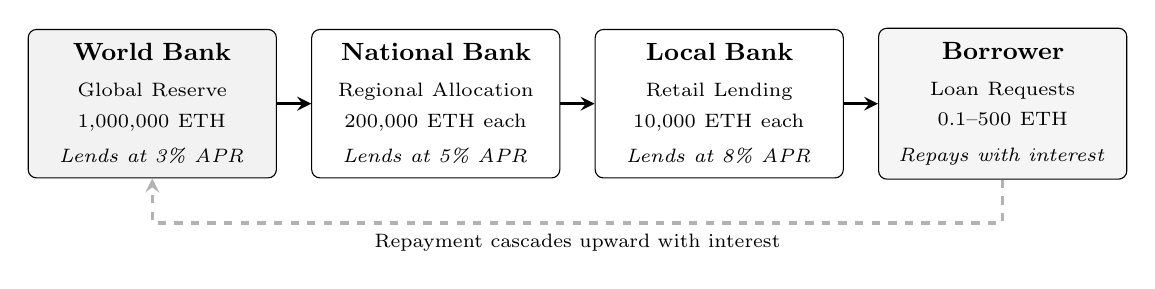
\begin{tikzpicture}[
    tier/.style={
        draw=black,
        fill=white,
        rounded corners=3pt,
        minimum width=3cm,
        minimum height=1.8cm,
        text width=2.8cm,
        align=center,
        font=\small,
        inner sep=5pt,
    },
    tierarrow/.style={
        ->,
        >=stealth,
        line width=1.2pt,
        color=black,
    },
]
\node[tier,fill=gray!10] (wb) at (0,0) {%
    \textbf{World Bank}\\[2pt]
    {\scriptsize Global Reserve}\\
    {\scriptsize 1,000,000 ETH}\\[2pt]
    {\scriptsize\textit{Lends at 3\% APR}}};

\node[tier] (nb) at (3.6,0) {%
    \textbf{National Bank}\\[2pt]
    {\scriptsize Regional Allocation}\\
    {\scriptsize 200,000 ETH each}\\[2pt]
    {\scriptsize\textit{Lends at 5\% APR}}};

\node[tier] (lb) at (7.2,0) {%
    \textbf{Local Bank}\\[2pt]
    {\scriptsize Retail Lending}\\
    {\scriptsize 10,000 ETH each}\\[2pt]
    {\scriptsize\textit{Lends at 8\% APR}}};

\node[tier,fill=gray!8] (br) at (10.8,0) {%
    \textbf{Borrower}\\[2pt]
    {\scriptsize Loan Requests}\\
    {\scriptsize 0.1--500 ETH}\\[2pt]
    {\scriptsize\textit{Repays with interest}}};

\draw[tierarrow] (wb) -- (nb);
\draw[tierarrow] (nb) -- (lb);
\draw[tierarrow] (lb) -- (br);

\draw[tierarrow,dashed,color=gray!60] (br.south) -- ++(0,-0.55) -| node[below,pos=0.25,font=\scriptsize,color=black] {Repayment cascades upward with interest} (wb.south);
\end{tikzpicture}
\caption{Four-tier hierarchical capital flow with cascading repayment.}
\label{fig:four-tier}
\end{figure}


\section{Auxiliary Dual-Currency Facility}

The cryptocurrency exchange feature of Crypto World Bank is built upon the cryptocurrency exchange facility that is an auxiliary facility incorporated into the current banking infrastructures all over the world. Instead of being a separate exchange, the platform is a service that is provided by all participating banks as an additional service to the existing product portfolio.

\begin{itemize}[noitemsep]
\item \textbf{Integration model:} The dual-currency facility is offered by all participating banks as an add-on service to their existing product portfolio. No additional banking license or separate entity is needed.
\item \textbf{Eligibility determination:} Eligibility of the dual-currency service is based on the bank officers managing the lending operations, on the basis of existing KYC/AML compliance, account status, and lending relationship history.
\item \textbf{No defaulting of conditions:} The project does not override, modify, or default any existing banking conditions, regulatory requirements, or contractual obligations.
\item \textbf{Scope:} The facility enables fiat-to-crypto and crypto-to-fiat conversions, cryptocurrency-denominated lending and repayment, and transparent on-chain transaction records---all within the governance structure of the participating bank.
\end{itemize}


\section{Governance Framework}

\subsection{Network Membership Governance}

\begin{table}[H]
\centering
\TableImageMaxFit{3.8.png}
\TableScreenshotEnd
\end{table}

\subsection{Business Network Governance}

\begin{table}[H]
\centering
\TableImageMaxFit{3.9.png}
\TableScreenshotEnd
\end{table}

\subsection{Technology Infrastructure Governance}

\begin{table}[H]
\centering
\TableImageMaxFit{3.10.png}
\TableScreenshotEnd
\end{table}

\subsection{Regulatory Compliance Considerations}

As the platform is active in the regulated banking sector:
\begin{itemize}[noitemsep]
\item Our prototype stage would be solely on the \textbf{public testnets} without attached real monetary value.
\item The architecture would facilitate \textbf{audit logs generation} to be reviewed by regulatory regimes on the sandbox programs.
\item Future production deployment would engage \textbf{regulatory sandbox programs} in target jurisdictions.
\end{itemize}

\subsection{Asset Tokenization}

\begin{itemize}[noitemsep]
\item \textbf{Current implementation:} The native blockchain currency (ETH/MATIC) is used as the reserve and loan currency.
\item \textbf{Planned extension:} Support for ERC-20 stablecoins (USDC, USDT) for lending operations in USD; tokenized collateral instruments for lending situations where there isn't enough collateral.
\end{itemize}


%% %%%%%%%%%%%%%%%%%%%%%%%%%%%%%%%%%%%%%%%%%%%%%%%%%%%%%%%%%%%%
%% CHAPTER 4: METHODOLOGY
%% %%%%%%%%%%%%%%%%%%%%%%%%%%%%%%%%%%%%%%%%%%%%%%%%%%%%%%%%%%%%
\chapter{Methodology}

This project and its planning have been structured in accordance with the \href{https://bcolbd.org/uploads/guideline/BLOCKCHAIN\%20OLYMPIAD\%20BANGLADESH\%20AI\%20Guideline.pdf}{Blockchain Olympiad Bangladesh AI guidelines}~[16] and the final-year project evaluation rubrics.

\section{Development Methodology}

We adopted a \textbf{lightweight Agile/Scrum} methodology tailored for an academic prototype with a fixed two-month development window. The iterative approach enables incremental delivery of demonstrable features while accommodating evolving requirements inherent in research-oriented development. Figure~\ref{fig:agile-process} illustrates our Agile process.

\begin{figure}[H]
\centering
\FigureImageMaxFit{Agile Process Diagram.png}
\caption{Agile/Scrum process diagram showing sprint cycles, backlog refinement, and iterative delivery within the 8-week development window.}
\label{fig:agile-process}
\end{figure}

Here's how we'll use Agile:
\begin{itemize}[noitemsep]
\item \textbf{Sprint Duration:} A period of 2 to 3 weeks is allocated for every sprint (3 sprints total).
\item \textbf{Team Size:} A group of two developers will be assigned (thesis project). The work will be focused on the thesis project.
\item \textbf{Weekly Sync:} A weekly gathering will occur to assess progress. Issues will be identified during these meetings. Plans will also be developed in these sessions alongside progress checks.
\item \textbf{Sprint Planning:} Planning for the sprint will take place for one hour at the beginning of every sprint.
\item \textbf{Sprint Review and Retrospective:} Reviewing work occurs at every sprint's conclusion. A discussion on lessons learned will be conducted for 30 minutes.
\end{itemize}

\section{Planned AI/ML Support}

The initial section of the thesis involves assistance from AI/ML. Fraud checks, detection of unusual activities and clarification of decisions in lending will be demonstrated. A reliance on an impeccable data system is unwelcome for this paper.

For now AI/ML will be simple:

\begin{itemize}[noitemsep]
\item \textbf{Fraud verification:} Utilizing Random Forest for assessing the risk of transactions. Risk is determined through an analysis by Random Forest.
\item \textbf{Anomaly detection:} Isolation Forest is recommended for detecting unusual wallet activities when data is limited. It's not necessary to have extensive data for this method to be effective.
\item \textbf{Explainability:} Utilizing SHAP will continue to provide insights into decision-making. Explanations will be offered for the reasoning behind decisions.
\end{itemize}

Building comprehensive datasets and preparing models for practical application will be postponed. The focus of the report emphasizes the setup of blockchain lending over developing a complete machine-learning initiative. A complete machine-learning project will not be undertaken at this time.

\begin{figure}[H]
\centering
\FigureImageMaxFit{4.2 agile window.png}
\caption{Agile development lifecycle --- 2-month window with three sprints.}
\end{figure}

\begin{figure}[H]
\centering
\FigureImageMaxFit{Methodology.png}
\caption{Technical development methodology: blockchain (Solidity), frontend (React, Wagmi, WalletConnect), backend (Express.js REST API, PostgreSQL), and AI/ML (Python, FastAPI, scikit-learn, Random Forest, SHAP) components across the three sprints.}
\label{fig:methodology-technical}
\end{figure}


\section{Sprint Plan and Deliverables}

\subsection{Sprint 1: Foundation and Core Banking (Weeks 1--3)}

\textbf{Sprint Goal:} Establish core blockchain infrastructure and hierarchical banking structure.

\begin{table}[H]
\centering
\TableImageMaxFit{4.1.png}
\TableScreenshotEnd
\end{table}

\begin{table}[H]
\centering
\TableImageMaxFit{4.2.png}
\TableScreenshotEnd
\end{table}

\textbf{Sprint 1 Total:} 42 story points. Deliverables: smart contracts deployed on testnet, basic frontend with wallet connection, database schema implemented, role-based access control, dashboard UI.


\subsection{Sprint 2: Lending Features and Communication (Weeks 4--6)}

\textbf{Sprint Goal:} Implement complete lending workflow and communication features.

\begin{table}[H]
\centering
\TableImageMaxFit{4.3.png}
\TableScreenshotEnd
\end{table}


\subsection{Sprint 3: AI/ML Security and Finalization (Weeks 7--8)}

\textbf{Sprint Goal:} Integrate AI/ML analytics, complete testing, and prepare documentation.

\begin{table}[H]
\centering
\TableImageMaxFit{4.4.png}
\TableScreenshotEnd
\end{table}

Figure~\ref{fig:sprint-submission} shows the sprint submission workflow.

\begin{figure}[H]
\centering
\FigureImageMaxFit{Sprint submission Diagram.png}
\caption{Sprint submission diagram showing the workflow from backlog refinement through development, testing, review, and delivery for each sprint cycle.}
\label{fig:sprint-submission}
\end{figure}


\section{SDLC Stage Mapping}

We map our Agile sprints to the seven stages of the Software Development Life Cycle (SDLC). Figure~\ref{fig:sdlc-mapping} illustrates this mapping.

\begin{table}[H]
\centering
\TableImageMaxFit{4.5.png}
\TableScreenshotEnd
\end{table}

\begin{figure}[H]
\centering
\FigureImageMaxFit{SDLC stage mapping.png}
\caption{SDLC stage mapping diagram showing alignment between the seven SDLC stages and our three-sprint Agile methodology.}
\label{fig:sdlc-mapping}
\end{figure}


\section{Design Decisions and Alternatives}

For each major design decision, we evaluated alternatives and justified selections based on technical criteria, ecosystem maturity, and project constraints. Figure~\ref{fig:design-decisions} visualizes these comparisons.

\begin{table}[H]
\centering
\TableImageMaxFit{4.6.png}
\TableScreenshotEnd
\end{table}

\begin{figure}[H]
\centering
\FigureImageMaxFit{Design Decisions and Alternatives Considered.png}
\caption{Design decisions and alternatives visualization across all major technology choices.}
\label{fig:design-decisions}
\end{figure}

\subsection{Justification of Selected Technologies}

\textbf{1st Choice Justifications:}

\begin{itemize}[noitemsep]
\item \textbf{Agile/Scrum} was necessary due to the project's evolving nature. Frequent updates to smart contract designs, user interface steps and AI/ML connections were required. Adopting Agile allows for plan alterations during brief work cycles effectively avoiding time and resource loss. Significance arises as new concepts emerge during the prototype development process.

\item \textbf{DApp + Off-chain AI} architecture allows intensive machine learning operations to occur outside the blockchain. Machine learning tasks are often run on the blockchain at a considerable expense occasionally exceeding \$100 for a single operation. Off-chain processing enables the use of rapid GPUs along with widely-used Python machine learning resources. Final lending choices are managed exclusively by smart contracts on-chain ensuring that trust is maintained in critical areas.

\item \textbf{React + TypeScript} is beneficial as many Web3 libraries such as Wagmi, RainbowKit, Viem, and ethers.js are supported seamlessly. A vast community of developers exceeding 10~million exists for React making it simpler to access assistance and solutions.

\item \textbf{EVM (Solidity)} is regarded as the most thoroughly examined smart contract system. Over \$100~billion is secured across various blockchains by it. Building and testing the project without incurring costs is possible with free test networks such as Sepolia and Amoy. Security tools provided by OpenZeppelin have been thoroughly tested to ensure the protection of contracts.

\item \textbf{MUI (Material Design~3)} provides ready-made components for typical banking interface designs. The package contains various items such as data tables, form checks and layouts for dashboards. Utilizing MUI results in a time saving of around 40\% compared to starting from scratch.

\item \textbf{Random Forest} performs effectively alongside SHAP's TreeExplainer which swiftly computes precise Shapley values for tree models. Precise calculations are essential for adhering to regulations concerning decision-making transparency. Avoiding approximate methods ensures explanations remain stable which prevents issues during audits.

\item \textbf{Isolation Forest} does not require labeled data for training. Labeled fraud samples are few making it suitable for DeFi lending. Anomalies in transactions are scored swiftly as it operates with a time complexity of $O(n \log n)$.

\item \textbf{SHAP} provides feature importance through solid mathematical foundations from game theory (Shapley values). Characteristics such as accuracy, management of absent data and consistency are not assured by tools like LIME. These properties assist in fulfilling emerging regulations for explainable decisions within financial services.

\item \textbf{PostgreSQL} effectively manages complex time-based queries. Borrowing limits can be checked over periods such as 6 months or 1 year. ACID compliance is fully supported to ensure financial data remains secure. It supports JSON which facilitates easy adjustments to the database structure during the prototyping phase.

\item \textbf{Vercel + Render} facilitates deploying the demo globally at no charge. A live prototype can be accessed without the necessity of a setup on personal computers. Supervisors, examiners and other individuals are not required to deal with installation issues.
\end{itemize}

\textbf{2nd Choice Justifications (Why Retained as Alternatives):}

\begin{itemize}[noitemsep]
\item \textbf{Incremental methodology} enables more predictable outcomes. Results from this method are often delivered with clarity and reliability. Adapting to changes arising from research is not a strength of this approach. Effectiveness occurs mainly in stable environments such as during the production phase.

\item \textbf{Hybrid with Oracle} architecture (e.g., Chainlink) enables machine learning predictions on-chain by utilizing oracle data. Increased trust is provided for AI decisions. However some delays (30--60 seconds per update) and additional costs (\$0.10--1.00 per call) are associated with the use of oracles. Availability hinges on the existence of third-party oracle services.

\item \textbf{Vue + TypeScript} is relatively straightforward to learn. Its Web3 tools such as vue-dapp are often considered less developed. Updates on wallet integration libraries are not abundant.

\item \textbf{Solana (Rust)} possesses the capability to process significantly more transactions each second (65,000 TPS) compared to Ethereum's 15 TPS. A smaller developer community is associated with it and the tools available are not as refined. Learning Rust is not easy for everyone. Completing the project in under 8 weeks is not achievable.

\item \textbf{Tailwind CSS} offers enhanced design flexibility through utility classes. Creating consistent banking-style UI patterns requires significant effort compared to the immediate solutions offered by MUI.

\item \textbf{XGBoost} frequently outperforms Random Forest in structured data evaluations. Approximate methods are utilized by its SHAP tool rather than precise tree computations. Explanations cannot be guaranteed to be consistent.

\item \textbf{Autoencoder} can capture complex non-linear anomaly patterns. A large volume of training data and precise tuning are required for its effectiveness. In contrast parameters are not necessary for Isolation Forest. It often suits simple prototypes that work with limited data.

\item \textbf{LIME} offers faster results. Explanations however lack stability. Different outcomes can arise from identical inputs on multiple checks as demonstrated by Adom et al.~[4].

\item \textbf{SQLite} is straightforward to set up. Multiple writes at one time are not supported. Advanced queries such as window functions and CTEs are not included for calculating borrowing limits.

\item \textbf{Localhost only} eliminates hosting dependencies. Sharing the project remotely or collaborating for testing is limited by this approach. Academic review won't benefit from such isolation.
\end{itemize}


\section{Design Patterns}

Our system uses three design patterns:

\begin{itemize}[noitemsep]
\item \textbf{Singleton:} A singleton means that each primary contract is established a single time. Only one version is utilized by all ensuring a unified source of truth. Not everyone can create multiple versions of the contract.

\item \textbf{Observer:} Contracts generate alerts whenever actions occur such as loan requests. These alerts are processed by a service that updates the database. Notifications are not ignored; they receive attention.

\item \textbf{Adapter:} An Adapter is utilized by the wallet component to function with various wallet types (like MetaMask). Different wallets that adhere to the EIP-1193 standards can be easily integrated.
\end{itemize}


\section{Software Testing Strategy}

We test in a few ways:

\begin{itemize}[noitemsep]
\item \textbf{Smart contract unit tests:} Numerous tests for smart contracts exist in our Hardhat environment. Over 12 tests are conducted to verify actions related to managing reserves, sign-ups, loans and access permissions. No scenarios such as depositing zero or executing disallowed actions are missed in these assessments.
\item \textbf{Integration testing:} Whole process checks are conducted for integration tests. Wallet connection, loan request, approval and repayment processes are evaluated on the network. No critical steps are excluded from the process.
\item \textbf{AI/ML module verification:} Ensuring functionality is vital for our fraud and unusual activity detectors. Results are generated by the integration of the detectors with the overall system.
\item \textbf{Frontend testing:} Website appearance is evaluated on Chrome, Firefox and mobile devices. Tests are conducted to ensure that functionality is maintained across various platforms.
\end{itemize}


%% %%%%%%%%%%%%%%%%%%%%%%%%%%%%%%%%%%%%%%%%%%%%%%%%%%%%%%%%%%%%
%% CHAPTER 5: MARKET ANALYSIS AND FEASIBILITY
%% %%%%%%%%%%%%%%%%%%%%%%%%%%%%%%%%%%%%%%%%%%%%%%%%%%%%%%%%%%%%
\chapter{Market Analysis and Feasibility}

\section{Market Sizing}

\begin{table}[H]
\centering
\TableImageMaxFit{5.1.png}
\TableScreenshotEnd
\end{table}

\vspace{4pt}
\noindent\textit{\small\textbf{Sources:} (a)~TAM: DefiLlama~[13] reports DeFi lending TVL exceeding \$55~billion; World Bank Migration and Development Brief~[26] values global remittances at \$860~billion annually; IFC~[20] estimates the MSME financing gap at \$4.5~trillion; (b)~SAM and SOM: project-derived estimates based on industry segmentation of institutional lending and regulatory sandbox addressable market~[18].}

Currently no organized lending system in DeFi exists. Simple shared pools are commonly utilized within DeFi. A functioning cross-border money transfer mechanism is not being provided by Ripple (\$847M daily)~[25] or JPMorgan Kinexys (\$3--7B daily)~[40]. Large organizations demonstrate a desire for blockchain to be utilized in financial matters. A lending system is being developed by the Crypto World Bank to create accessibility similar to DeFi while also incorporating traditional banking structures aimed at fostering growth. No existing solution completely meets this need.

\section{Target Customer Segment}

The Crypto World Bank targets the \textbf{retail customer segment}---individual borrowers and small businesses seeking transparent, accessible crypto-based lending services.

\begin{table}[H]
\centering
\TableImageMaxFit{5.2.png}
\TableScreenshotEnd
\end{table}

\section{Partner Ecosystem}

\begin{table}[H]
\centering
\TableImageMaxFit{5.3.png}
\TableScreenshotEnd
\end{table}


\section{Competitive Landscape}

The Crypto World Bank operates at the intersection of four distinct competitor categories. Table~\ref{tab:competitor-detailed} provides a detailed comparison of representative projects in each category, with current metrics as of March~2026.

\begin{table}[H]
\centering
\TableImageMaxFit{5.4.1.png}
\TableScreenshotEnd[tab:competitor-detailed]
\end{table}

\begin{table}[H]
\centering
\TableImageMaxFit{5.4.2.png}
\TableScreenshotEnd
\end{table}

\begin{table}[H]
\centering
\TableImageMaxFit{5.4.3.png}
\TableScreenshotEnd
\end{table}

Upon reviewing various projects a common feature was identified: a lending mechanism does not exist that operates with tiers, is distributed and facilitates transactions across different levels and within identical levels. Such innovation distinguishes the Crypto World Bank. Here's why it's different:

\begin{itemize}[noitemsep]
\item Online lending in DeFi provides opportunities yet lacks a comprehensive framework. A defined structure is absent within the realm of DeFi lending.
\item Credit platforms such as Maple and Goldfinch engage in lending based on credit. Credit-based lending is often focused on businesses and exists at just one tier. These platforms do not cater to personal loans.
\item Payments are processed by banking systems such as Ripple. Lending and deposit services are not provided by this system. Ripple specializes in payment processing rather than other banking services.
\item Celo provides assistance to individuals in emerging economies. Payment and savings functions are offered yet lending services remain absent.
\item \textbf{Central Bank Digital Currencies (CBDCs):} The development of CBDCs aims to improve payment systems~[5]. Concerns about privacy and control are raised as lending features are excluded. A lending layer does not exist on a CBDC. Users benefit from our platform which safeguards their interests while providing a level-based system similar to that utilized by CBDCs~[45].
\end{itemize}

\section{Risk Taxonomy}

\begin{table}[H]
\centering
\TableImageMaxFit{5.5.png}
\TableScreenshotEnd
\end{table}


\section{Technical Feasibility}

\begin{table}[H]
\centering
\TableImageMaxFit{5.6.png}
\TableScreenshotEnd
\end{table}


\section{Economic Feasibility}

\begin{table}[H]
\centering
\TableImageMaxFit{5.7.png}
\TableScreenshotEnd
\end{table}


\section{Revenue Projection}

The following projection models annual revenue potential at full deployment scale. Calculations use a reference ETH price of \textbf{\$2,000} (February 2026 market rate) and interest rate parameters defined in Section~\ref{sec:interest-rates}.

\begin{table}[H]
\centering
\TableImageMaxFit{5.8.png}
\TableScreenshotEnd
\end{table}

\begin{table}[H]
\centering
\TableImageMaxFit{5.9.png}
\TableScreenshotEnd
\end{table}

\vspace{4pt}
\noindent\textit{\small\textbf{Sources:} ETH price from spot market data (CoinGecko); interest rate tiers aligned with Aave~[15] and Compound~[16] DeFi benchmarks; default rate and origination fee from conservative industry estimates.}

\vspace{6pt}
\noindent\textbf{Cost Model Considerations.} Considerations for the cost model require careful thought. Important aspects need to be addressed by the team. Various factors will certainly influence the overall calculation:

\begin{itemize}[noitemsep]
\item \textbf{Gas costs:} Gas expenses on Polygon PoS are quite low. A loan's entire process including request, approval, payment and 12 monthly installments results in costs under \$0.15. Interest income amounts to less than 0.01\% of our earnings. For Ethereum, loan costs may range from \$50 to \$750 influenced by network congestion. Processing transactions in batches or utilizing Layer~2 would be essential for the viability of small loans.
\item \textbf{Infrastructure costs:} Backend hosting (API server, database, ML service), frontend delivery (CDN) and RPC nodes (Alchemy, Infura) can incur costs ranging between \$500 and \$2,000 monthly. An increase in expenses will be experienced with a rise in transactions.
\item \textbf{Default losses:} A default rate of 3\% is anticipated. Approximately \$6.7~million annually is projected as the platform sees heavy usage. Anticipated earnings have already incorporated this amount.
\item \textbf{Break-even analysis:} Opportunities for profit on loans as small as 0.01~ETH (\$20) exist on Polygon PoS. Profitability on loans below 5~ETH (\$10,000) is not achievable on Ethereum without Layer~2. Layer~2 is essential for facilitating small loans.
\end{itemize}

\begin{figure}[H]
\centering
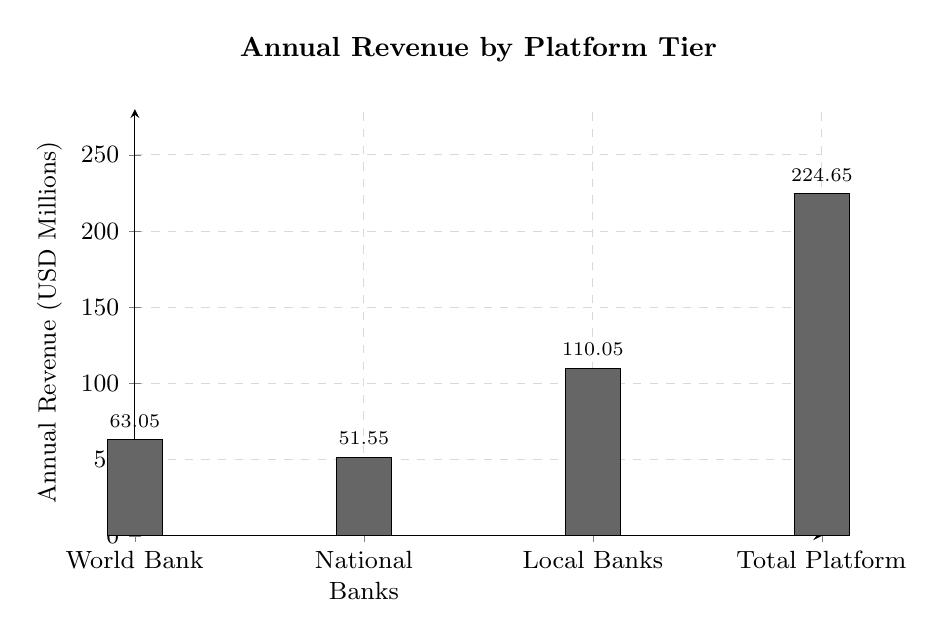
\begin{tikzpicture}
\begin{axis}[
    ybar,
    bar width=20pt,
    width=0.85\textwidth,
    height=7cm,
    clip=false,
    ylabel={Annual Revenue (USD Millions)},
    ylabel style={font=\small},
    symbolic x coords={World Bank,National Banks,Local Banks,Total Platform},
    xtick=data,
    xticklabel style={font=\small,text width=2.2cm,align=center},
    yticklabel style={font=\small},
    ymin=0,
    ymax=280,
    ytick={0,50,100,150,200,250},
    nodes near coords,
    nodes near coords style={font=\scriptsize\bfseries},
    every node near coord/.append style={anchor=south,yshift=1pt},
    enlarge x limits=0.30,
    grid=major,
    grid style={dashed,gray!30},
    axis lines=left,
    title={\textbf{Annual Revenue by Platform Tier}},
    title style={font=\normalsize,at={(0.5,1.05)}},
]
\addplot[fill=black!60,draw=black] coordinates {
    (World Bank,63.05) (National Banks,51.55) (Local Banks,110.05) (Total Platform,224.65)
};
\end{axis}
\end{tikzpicture}
\caption{Annual revenue projection by tier (USD millions, at \$2{,}000/ETH).}
\end{figure}

\subsection{Transaction Economics: Interest Rates}
\label{sec:interest-rates}

\begin{table}[H]
\centering
\TableImageMaxFit{5.10.png}
\TableScreenshotEnd
\end{table}

\begin{figure}[H]
\centering
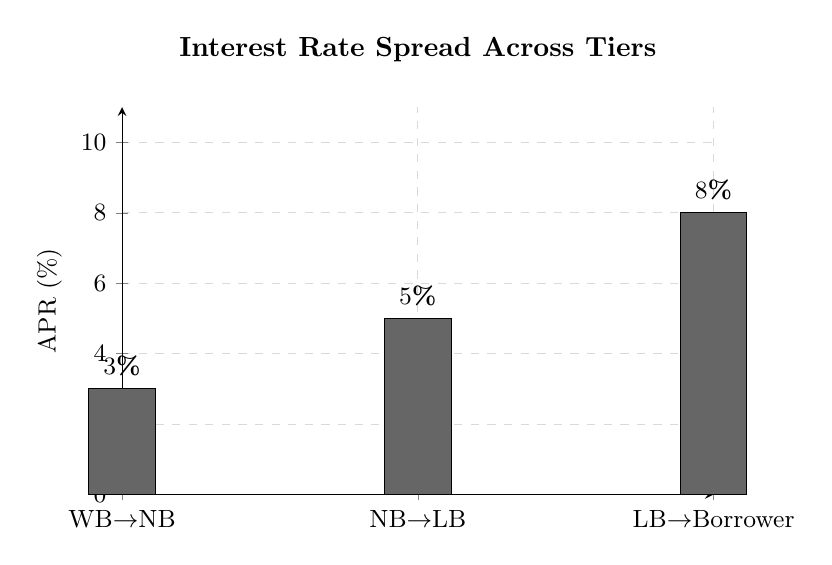
\begin{tikzpicture}
\begin{axis}[
    ybar,
    bar width=24pt,
    width=0.75\textwidth,
    height=6.5cm,
    clip=false,
    ylabel={APR (\%)},
    ylabel style={font=\small},
    symbolic x coords={WB$\to$NB,NB$\to$LB,LB$\to$Borrower},
    xtick=data,
    xticklabel style={font=\small},
    yticklabel style={font=\small},
    ymin=0,
    ymax=11,
    ytick={0,2,4,6,8,10},
    nodes near coords={\pgfmathprintnumber\pgfplotspointmeta\%},
    nodes near coords style={font=\small\bfseries},
    every node near coord/.append style={anchor=south,yshift=1pt},
    enlarge x limits=0.50,
    grid=major,
    grid style={dashed,gray!30},
    axis lines=left,
    title={\textbf{Interest Rate Spread Across Tiers}},
    title style={font=\normalsize,at={(0.5,1.05)}},
]
\addplot[fill=black!60,draw=black] coordinates {
    (WB$\to$NB,3) (NB$\to$LB,5) (LB$\to$Borrower,8)
};
\end{axis}
\end{tikzpicture}
\caption{Hierarchical interest rate spread (APR) across the four-tier lending structure.}
\end{figure}

\subsection{Global Economic Impact}

Apart from revenue generated through platforms, various economic advantages are provided by the Crypto World Bank:

\begin{itemize}[noitemsep]
\item \textbf{Capital deployment and fiscal multiplier:} Funding efforts have been made by the Crypto World Bank specifically targeting developing nations. A sum of \$2~billion has been provided to nearly 1,000 borrowers. Loans from substantial institutions do not merely generate a single dollar; they generate approximately \$2.5 to \$3 in additional economic growth~[19]. A significant increase in the economy estimated at \$5 to \$6~billion annually may be driven by lending practices. Approximately 16 new jobs are created in developing nations for every \$1~million lent to small businesses as shown by IFC~[20].

\item \textbf{Remittance cost reduction:} Annually approximately \$860~billion is transferred globally as remittances. A significant portion of this estimated between \$48 and \$56~billion is lost through transfer fees. Average fees are not less than 6.49\% exceeding the United Nations target of 3\% by more than double~[26]. On-chain settlement, a rapid blockchain technique, is utilized by the Crypto World Bank to reduce costs to under 1\%. Annually payments amounting to \$55.6~billion are processed by Stellar incurring minimal fees around \$0.0007 per transaction~[44]. Payments are processed by Celo's MiniPay for under a cent across more than 60 nations~[42].

\item \textbf{Trapped capital liberation:} Trapped capital can now be released. Money is required by banks to remain in nostro and vostro accounts for international transactions~[24]. Pre-funded accounts are no longer necessary due to the rapid payment settlements provided by the Crypto World Bank's blockchain system. Increased funds become available for lending purposes.

\item \textbf{Financial inclusion:} Focused on financial inclusion, the platform caters to regular users. Features such as zero gas fees for transactions, optimized mobile performance, and the option to lend tiny sums below one dollar are provided. Credit remains uncomplicated and accessible for the 1.4~billion individuals globally who lack banking services~[14]. A ``leapfrog technology'' is how decentralized finance (DeFi) has been described by the World Economic Forum serving to assist individuals in bypassing conventional banks~[41]. In numerous developing nations mobile phones have overtaken landlines showcasing a significant shift in technology.

\item \textbf{Transaction cost reduction:} Transaction expenses are significantly reduced. Fees on the Polygon PoS network remain below one cent resulting in over a \textbf{99\% reduction} from the average \$42 transaction fee seen in traditional correspondent banking systems~[25]. Many small transactions which weren't feasible previously are now possible due to this substantial decrease in costs.

\item \textbf{Transparency as an economic good:} Clarity serves as an advantage. Reserve amounts, interest rates and transaction records are displayed on the blockchain. Harmful practices such as predatory lending are not enabled by this transparency; borrowers are less likely to face unfair charges or hidden fees. Information imbalance in traditional banking does not always favor borrowers particularly in developing countries resulting in disadvantageous agreements. Through the Crypto World Bank's platform, identical information can be viewed and verified by all participants promoting fairness and honesty in lending.
\end{itemize}

\subsection{Value Proposition and Go-to-Market}

\begin{table}[H]
\centering
\TableImageMaxFit{5.11.png}
\TableScreenshotEnd
\end{table}


\section{Prototype Scope and Limitations}

A straightforward version of the complete system is represented by the current prototype:

\begin{enumerate}[noitemsep]
\item \textbf{Hierarchical lending scope:} Utilization of the Tier~1 World Bank Reserve contract is comprehensive. Deposits are managed, loan requests and approvals are processed alongside the display of reserve statistics. Not all functions of the Tier~2 (National Bank) and Tier~3 (Local Bank) contracts have been implemented. Role management and registration are not the only aspects focused on. Currently the process for fund transfers from the World Bank to National Bank and subsequently to Local Bank is incomplete. Four tiers will be included in the final design.

\item \textbf{Interest accrual and repayment:} Rules for interest rates (3\%/5\%/8\%) are part of the system design. Fees for initiating loans and penalties for delays also exist. Interest calculations, payment schedules or penalties aren't managed automatically by current smart contracts. Future updates will incorporate these functions.

\item \textbf{InterBankLendingPool and multi-directional flows:} Plans for interbank loans at equal tier levels are included in the design (Section~1.7). Smart contracts have yet to be created for those components. Currently the prototype does not prioritize the upward transfer of funds.

\item \textbf{AI/ML integration:} AI tools such as fraud detection (Random Forest) and anomaly detection (Isolation Forest) along with decision explanations (SHAP) are set to be utilized by the system. A service has been established with FastAPI for machine learning. This service does not currently link to the loan approval process in the existing version.

\item \textbf{Backend architecture:} Express.js paired with MongoDB is utilized for rapid API development. The main database is intended to be PostgreSQL. FastAPI is utilized by the machine learning service.
\end{enumerate}

Normal limits exist for the initial phase of the project. The design of the system and the establishment of basic infrastructure are prioritized during this stage. All features will not be included in this part. The complete system will be created in the subsequent phase.


%% %%%%%%%%%%%%%%%%%%%%%%%%%%%%%%%%%%%%%%%%%%%%%%%%%%%%%%%%%%%%
%% CHAPTER 6: CONCLUSION
%% %%%%%%%%%%%%%%%%%%%%%%%%%%%%%%%%%%%%%%%%%%%%%%%%%%%%%%%%%%%%
\chapter{Conclusion}

The Crypto World Bank deals with a \textbf{multi-party, multi-party coordination and trust} issue in hierarchical development finance through exploitation of the special features of blockchain technology: cryptographic, immutability, and programmable auditability. Our solution is better than the current DeFi lending protocols---which collectively manage over \$55~billion of TVL~[13] and everywhere use flat and single-tier pool architectures---through a four tier institutional hierarchy with cross-tier, same-tier and upward lending flows, along with a governance structure that deals with network membership, business operations and technology infrastructure.

The analysis of the competitive situation of 20+ existing projects in DeFi lending, institutional credit, banking infrastructure and financial inclusion affirm that no current system is a combination of multi-level lending (hierarchy), interbank lending mechanisms and graded access by borrowers in one decentralized architecture. The growing blockchain implementation in the institutions, as demonstrated by the World Bank FundsChain initiative~[39], the multi-billion-dollar daily volumes of JPMorgan Kinexys~[40] and R3 Corda's \$17~billion in tokenized assets~[37]---validates both the technical feasibility and institutional demand of blockchain-based financial infrastructure. The Crypto World Bank takes this trend of settlement and fund tracking to the fullest open and hierarchical lending structure.

The site is located on the border of institutional and decentralized finance lending, and financial inclusion---a mix, which is currently unaddressed in both the scholarly literature and the business blockchain environment. With a working prototype, a defined market and partnership plan, and a planned go-to-market plan, the Crypto World Bank is a possible and scalable addition to the new field of blockchain-based development finance.

The future work will be directed towards the following directions:

\begin{enumerate}[noitemsep]
\item \textbf{Complete hierarchical lending implementation:} Complete the end-to-end wiring of cross-tier fund transfers between the World Bank Reserve, National Bank and Local Bank contracts, including automated capital distribution, interest accrual, generation of installments schedules, generation of cascading repayments enforcement as intended in the architecture.
\item \textbf{InterBankLendingPool and multi-directional flows:} Adopt the same-tier interbank lending pool and upward surplus repatriation mechanisms described in Section~1.7, so as to permit a full modeling of real-life banking liquidity flows in the decentralized structure.
\item \textbf{AI/ML pipeline integration:} Integrate the ML inference based on FastAPI service (Random Forest fraud detection, Isolation Forest anomaly detection, SHAP explainability) into the real-life loan approval process, integrating off-chain on-chain lending decisions to risk assessments.
\item \textbf{Mainnet and regulatory sandbox:} Moving off the testnet to the mainnet featuring real asset testing in regulated sandbox settings (e.g. UK FCA Digital Securities Sandbox, MAS FinTech Regulatory Sandbox Singapore, Bangladesh Bank FinTech Regulatory Sandbox).
\item \textbf{Extended surveillance assistance:} More developed risk-monitoring and anomaly detection modules can be considered in the following phases after the main lending workflow has been developed and blockchain architecture is completely stabilized.
\item \textbf{Cross-chain interoperability:} Ethereum Layer~2 multi-network lending rollups (Arbitrum, Optimism, Base) and other EVM chains to serve other geographic markets having optimized gas costs and local regulatory compliance.
\item \textbf{Formal security checking:} Formal verification of all smart contract code based on symbolic execution (Mythril), and static analysis (Slither), formal verification of property (Certora), especially multi-tier lending invariants such as cascading reserve ratio maintenance and cross-tier interest rate bound enforcement.
\item \textbf{Stablecoin integration, fiat on/off-ramps:} Support established blockchain coins (USDC, USDT, DAI) and native blockchain coins, with fiat on/off-ramping by collaborating with licensed money transmitters or anchor networks like MoneyGram that Stellar has implemented~[44].
\item \textbf{Economic simulation and stress testing:} Agent-based simulation of the hierarchical lending system under market stress conditions (bank runs, cascading liquidations, correlated collateral devaluation) to prove convergence of interest rates, adequacy in the reserve ratios, and stability in the system.
\end{enumerate}


%% %%%%%%%%%%%%%%%%%%%%%%%%%%%%%%%%%%%%%%%%%%%%%%%%%%%%%%%%%%%%
%% APPENDICES
%% %%%%%%%%%%%%%%%%%%%%%%%%%%%%%%%%%%%%%%%%%%%%%%%%%%%%%%%%%%%%
\appendix

\chapter{Technology Stack}

\section{In-product assistant: local large language model (LLM) integration (prototype)}

\paragraph{Purpose.}
The web application includes a streaming chat assistant to help users understand platform concepts (e.g., the four-tier capital hierarchy), screen-specific workflows, and navigation. During local development, the assistant is served by a \textbf{local OpenAI-compatible inference server} (LM Studio) running a quantized Gemma-family model, while the public browser traffic is still routed through the project API to keep keys off the client and to centralize request shaping (system prompts, optional authenticated user context, and error handling).

\paragraph{Model and runtime (local development).}
The inference endpoint follows the \textbf{OpenAI Chat Completions} contract (\texttt{/v1/chat/completions}) with \texttt{stream: true}, proxied from the project backend to a local service such as \texttt{http://127.0.0.1:1234}. The served checkpoint is configured as a Gemma-4 E4B variant (e.g., \texttt{google/gemma-4-e4b}) in GGUF form with a practical quantization (e.g., \texttt{Q4\_K\_M}) for a laptop-friendly footprint (on the order of single-digit GBs). The exact quantization label and on-disk name are a deployment artifact; what matters for integration is the \textbf{API model identifier} exposed by the local server and referenced by the backend configuration (environment-driven).

\paragraph{End-to-end behavior.}
The user interface assembles a short transcript (user/assistant messages) and posts it to the backend streaming route. The backend prepends a \textbf{system message} with platform + screen ``feature'' context, optionally enriched by user role when a valid session token is present. The backend then opens a streaming request to the local model server, converts upstream token events into \textbf{server-sent events (SSE)} for the browser, and the UI incrementally appends text. The message renderer uses Markdown (including GitHub-flavored extensions), math (KaTeX) for \texttt{\$\$...\$\$} blocks, and line-break rules appropriate for chat transcripts.

\paragraph{Security and limitations (prototype stance).}
The assistant is a \textbf{read-only product guide}: it is not an authoritative source of on-chain truth and it does not sign transactions. Hallucination risk exists; production hardening would add retrieval of verified platform facts and stronger safety policies. The implementation prioritizes \textbf{developer ergonomics} (local model, same-machine loop) over maximum isolation boundaries.

\paragraph{Architecture diagram (Mermaid).}
Mermaid is convenient for version-control-friendly diagrams, but a typical \texttt{pdflatex} build does not render Mermaid natively. Figure~\ref{fig:local-llm-mermaid} therefore includes the Mermaid \emph{source} for reproducibility, while Figure~\ref{fig:local-llm-tikz} provides an equivalent, PDF-safe TikZ view for the report compilation pipeline used here.

\begin{figure}[H]
\centering
\begin{tcolorbox}[colback=LightBlue,colframe=PrimaryBlue!35!white,boxrule=0.8pt,arc=3pt,left=4pt,right=4pt,top=4pt,bottom=4pt]
\small
\begin{verbatim}
flowchart TB
  subgraph UI["Web UI (Vite + React)"]
    L["Landing assistant (public)"]
    A["In-app: floating widget + /app/assistant page"]
    R["Message rendering: Markdown + math (KaTeX) + line breaks"]
    Q["Feature-aware quick prompts: route -> featureKey -> suggestions"]
  end

  subgraph DEV["Vite dev proxy (local only)"]
    P["/api -> http://127.0.0.1:4000 (same origin in the browser)"]
  end

  subgraph API["CWB API (Express)"]
    S["POST /api/ai/chat/stream (SSE)"]
    OA["optionalAuth: if Authorization Bearer -> session user/role (else anonymous)"]
    SP["Assemble: system instructions + (optional) user context + chat transcript + featureKey/route"]
  end

  subgraph LLM["Local inference (LM Studio)"]
    O["OpenAI-compatible server: http://127.0.0.1:1234"]
    C["POST /v1/chat/completions (stream=true)"]
  end

  Q --> L
  Q --> A
  L --> R
  A --> R

  L -->|fetch: POST /api/ai/chat/stream| P
  A -->|fetch: POST /api/ai/chat/stream| P
  P --> S
  S --> OA
  OA --> SP
  SP -->|upstream: streaming chat completions| O
  O --> C
  C -- "server emits token deltas (stream)" --> SP
  SP -- "SSE to browser: event token/meta/done" --> P
  P -- "incremental text + replace loading bubble" --> R
\end{verbatim}
\end{tcolorbox}
\caption{Mermaid source for the local LLM chatbot integration (browser $\rightarrow$ API $\rightarrow$ local OpenAI-compatible model server, streaming).}
\label{fig:local-llm-mermaid}
\end{figure}

\begin{figure}[H]
\centering
\begin{tikzpicture}[
  font=\small,
  node distance=8mm and 10mm,
  box/.style={draw=PrimaryBlue!70, rounded corners=3pt, align=left, inner sep=6pt, fill=LightBlue},
  server/.style={draw=GreenAccent!70!black, rounded corners=3pt, align=left, inner sep=6pt, fill=RowShade},
  smalllabel/.style={font=\scriptsize, inner sep=1pt, fill=white, draw=none},
  -{Stealth[length=2.2mm]}
]

\node[box, text width=0.44\linewidth] (ui) {%
  \textbf{Web UI (Vite + React)}\\
  \textbullet\ Landing assistant (public)\\
  \textbullet\ In-app assistant widget + full page (\texttt{/app/assistant})
};

\node[box, text width=0.40\linewidth, right=6mm of ui] (api) {%
  \textbf{CWB API (Express)}\\
  \texttt{POST /api/ai/chat/stream} (SSE)\\
  \textbullet\ \textbf{optionalAuth:} accept JWT if present\\
  \textbullet\ \textbf{Prompt shaping:} system + feature context
};

\node[server, text width=0.40\linewidth, below=12mm of api, anchor=north] (lm) {%
  \textbf{Local inference (LM Studio)}\\
  \texttt{http://127.0.0.1:1234}\\
  \texttt{POST /v1/chat/completions} (stream)\\
  \textbullet\ OpenAI-compatible chat schema
};

\draw[->] (ui.east) -- node[smalllabel, pos=0.5, sloped, above=1pt] {HTTP: transcript + feature context} (api.west);
\draw[->] (api.south) -- node[smalllabel, pos=0.5, right=1pt] {upstream: chat completions} (lm.north);
\draw[->, Stealth-Stealth] (lm.west) .. controls +(-0.6,0) and +(-0.6,0) .. node[smalllabel, pos=0.5, left=1pt] {SSE: tokens + metadata} (ui.west);

\end{tikzpicture}
\caption{Local LLM assistant data flow: browser UI streams from the CWB API, which proxies to a local OpenAI-compatible model server. The path is the same in principle for both landing and in-app UIs, with optional user context when authenticated.}
\label{fig:local-llm-tikz}
\end{figure}

\paragraph{Implementation analysis (brief).}
The integration is successful for the project prototype because it reuses a stable transport shape (chat-completions with streaming) and isolates the model vendor behind a single API route, allowing the user interface to remain a thin client. The main practical engineering challenges in local development were: (1) \textbf{process/port hygiene} to keep the API bound to a predictable port, (2) \textbf{CORS and same-origin} considerations when the UI and API run on different localhost ports, mitigated with a Vite dev proxy to \texttt{/api} and with permissive dev CORS policy on the API, and (3) \textbf{RPC provider selection} for wallet reads in the browser, where some public endpoints may fail browser CORS; pinning explicit public RPC endpoints avoids noisy failures unrelated to the chat feature.

\paragraph{Relationship to the earlier rule-based assistant (legacy).}
The repository also retains early keyword-routed \texttt{/api/chatbot} handlers used for initial prototyping; the LLM path is additive. This separation prevents regressions in deterministic demo endpoints while the conversational assistant evolves.

\begin{table}[H]
\centering
\TableImageMaxFit{table A.1.png}
\TableScreenshotEnd
\end{table}

\chapter{Smart Contract Capabilities}

The three smart contracts of the platform assist in the following operations:

\begin{itemize}[noitemsep]
\item \textbf{World Bank Reserve Contract:} Reserving, deposit handling, national bank registration, fund allocation to the national banks, system pause/unpause, emergency withdrawal and world statistics.
\item \textbf{National Bank Contract:} Local bank registration, borrowing the world bank reserve, fund allocation to local banks, and network stature queries.
\item \textbf{Local Bank Contract:} Installment, loan approval and denial, loan request payments, management of bank users as well as approver designation.
\end{itemize}


%% %%%%%%%%%%%%%%%%%%%%%%%%%%%%%%%%%%%%%%%%%%%%%%%%%%%%%%%%%%%%
%% REFERENCES
%% %%%%%%%%%%%%%%%%%%%%%%%%%%%%%%%%%%%%%%%%%%%%%%%%%%%%%%%%%%%%
\chapter*{References}
\addcontentsline{toc}{chapter}{References}

{\small
\begin{enumerate}[label={[\arabic*]}]
\item S.~M. Werner, D.~Perez, L.~Gudgeon, A.~Klages-Mundt, D.~Harz, and W.~J. Knottenbelt, ``SoK: Decentralized Finance (DeFi),'' \textit{arXiv preprint arXiv:2101.08778}, 2022. [Online]. Available: \url{https://arxiv.org/abs/2101.08778}

\item S.~Bastankhah, M.~Hashemi, and W.~Shi, ``An Adaptive Data-Driven DeFi Borrow-Lending Protocol,'' \textit{Proc. IEEE Int. Conf. Blockchain}, 2023.

\item G.~Palaiokrassas, A.~Skoufis, and L.~Tassiulas, ``Leveraging Machine Learning for Multichain DeFi Fraud Detection,'' \textit{Proc. IEEE Int. Conf. Blockchain and Cryptocurrency (ICBC)}, 2023.

\item D.~Adom, E.~O. Acheampong, and M.~Boateng, ``LIME and SHAP: A Comparison of Model-Agnostic Approaches to Explainability in Loan Approval Systems,'' \textit{International Journal of Advanced Computer Science and Applications}, vol.~13, no.~11, 2022.

\item B.~W. Tan, ``Central Bank Digital Currency and Financial Inclusion,'' \textit{IMF Working Paper WP/23/69}, 2023. [Online]. Available: \url{https://www.imf.org/en/Publications/WP}

\item F.~T. Liu, K.~M. Ting, and Z.-H. Zhou, ``Isolation Forest,'' in \textit{Proc. IEEE Int. Conf. Data Mining (ICDM)}, pp.~413--422, 2008. DOI: \url{https://doi.org/10.1109/ICDM.2008.17}

\item N.~Atzei, M.~Bartoletti, and T.~Cimoli, ``A Survey of Attacks on Ethereum Smart Contracts (SoK),'' in \textit{Proc. Int. Conf. Principles of Security and Trust (POST)}, pp.~164--186, 2017. DOI: \url{https://doi.org/10.1007/978-3-662-54455-6_8}

\item S.~M. Lundberg and S.-I. Lee, ``A Unified Approach to Interpreting Model Predictions,'' in \textit{Advances in Neural Information Processing Systems (NeurIPS)}, pp.~4765--4774, 2017. [Online]. Available: \url{https://proceedings.neurips.cc/paper/2017/hash/8a20a8621978632d76c43dfd28b67767-Abstract.html}

\item P.~Bracke, A.~Datta, C.~Jung, and S.~Sen, ``Machine Learning Explainability in Finance: An Application to Default Risk Analysis,'' \textit{Bank of England Staff Working Paper No.~816}, 2019. [Online]. Available: \url{https://www.bankofengland.co.uk/working-paper/2019/machine-learning-explainability-in-finance}

\item R.~Beck, C.~M\"{u}ller-Bloch, and J.~L. King, ``Governance in the Blockchain Economy: A Framework and Research Agenda,'' \textit{Journal of the Association for Information Systems}, vol.~19, no.~10, pp.~1020--1034, 2018. DOI: \url{https://doi.org/10.17705/1jais.00518}

\item D.~Mhlanga, ``Blockchain Technology for Financial Inclusion and Sustainable Development,'' in \textit{Digital Financial Inclusion}, Springer, 2022.

\item OpenZeppelin, ``OpenZeppelin Contracts,'' 2024. [Online]. Available: \url{https://openzeppelin.com/contracts}

\item DefiLlama, ``Lending Protocols --- DeFi TVL and Protocol Rankings,'' 2024--2025. [Online]. Available: \url{https://defillama.com/protocols/lending}

\item World Bank, ``The Global Findex Database 2021: Financial Inclusion, Digital Payments, and Resilience,'' 2021. [Online]. Available: \url{https://www.worldbank.org/en/publication/globalfindex}

\item Aave, ``Aave Protocol Documentation,'' 2024. [Online]. Available: \url{https://docs.aave.com/}

\item Compound, ``Compound Protocol Documentation,'' 2024. [Online]. Available: \url{https://docs.compound.finance/}

\item BCOLBD 2025, ``Blockchain Olympiad Bangladesh: Guideline and Evaluation Scheme,'' 2025. [Online]. Available: \url{https://bcolbd.org/uploads/guideline/BLOCKCHAIN\%20OLYMPIAD\%20BANGLADESH\%20Blockchain\%20Guideline.pdf}

\item Galaxy Digital, ``The State of Crypto Lending and Borrowing,'' Galaxy Research, 2024. [Online]. Available: \url{https://www.galaxy.com/insights/research/the-state-of-crypto-lending}

\item World Bank, ``World Development Report 2022: Finance for an Equitable Recovery,'' 2022. [Online]. Available: \url{https://www.worldbank.org/en/publication/wdr2022}

\item International Finance Corporation (IFC), ``MSME Finance Gap 2019,'' 2019. [Online]. Available: \url{https://www.ifc.org/en/insights-reports/2019/msme-finance-gap}

\item Bank for International Settlements, ``DeFi Lending: Intermediation Without Information?,'' BIS Working Paper No.~1183, 2024. [Online]. Available: \url{https://www.bis.org/publ/work1183.pdf}

\item Deloitte, ``Global Banking Outlook 2024,'' 2024.

\item Michigan State University Libraries, ``Literature Table and Synthesis --- Nursing Literature Reviews,'' LibGuides, 2025. [Online]. Available: \url{https://libguides.lib.msu.edu/nursinglitreview/table}

\item Committee on Payments and Market Infrastructures and Bank for International Settlements, ``Correspondent Banking --- Technical Report,'' CPMI Papers No.~147, 2016. [Online]. Available: \url{https://www.bis.org/cpmi/publ/d147.pdf}

\item Ripple, ``RLUSD Use Case Analysis,'' XRP Academy, 2026. [Online]. Available: \url{https://xrpacademy.com/blog/rlusd-use-case-analysis-calendar-570}

\item World Bank, ``Remittance Prices Worldwide: Making Markets More Transparent,'' Migration and Development Brief~40, 2024. [Online]. Available: \url{https://remittanceprices.worldbank.org/}

\item DefiLlama, ``Aave V3 TVL, Fees, Revenue \& Income Statement,'' March 2026. [Online]. Available: \url{https://defillama.com/protocol/aave-v3}

\item World Inequality Lab, ``Exorbitant Privilege,'' \textit{World Inequality Report 2026}, 2026. [Online]. Available: \url{https://wir2026.wid.world/insight/exorbitant-privilege/}

\item DefiLlama, ``Compound V3 TVL, Fees, Revenue \& Income Statement,'' March 2026. [Online]. Available: \url{https://defillama.com/protocol/compound-v3}

\item Fensory, ``Sky Protocol Projects \$611M Revenue in 2026 as USDS Supply Targets \$20.6 Billion,'' February 2026. [Online]. Available: \url{https://www.fensory.com/intelligence/rwa/sky-protocol-tokenization-regatta-solana-february-2026}

\item Fensory, ``Maple Finance --- Institutional DeFi Lending Protocol,'' 2026. [Online]. Available: \url{https://www.fensory.com/insights/protocols/maple-finance}

\item Fensory, ``DeFi Credit Platforms Hit \$2.4B Milestone,'' March 2026. [Online]. Available: \url{https://www.fensory.com/intelligence/rwa/defi-private-credit-platforms-2-4-billion-loans-ethereum}

\item Financial Stability Board, ``Enhancing Cross-border Payments: Stage 3 Roadmap,'' 2020. [Online]. Available: \url{https://www.fsb.org/2020/10/enhancing-cross-border-payments-stage-3-roadmap/}

\item A.~Beyer, B.~Gasperini, and P.~Theodoridis, ``Monetary Policy and Inequality: Distributional Effects of Asset Purchase Programs,'' \textit{Journal of International Money and Finance}, vol.~157, 2025.

\item Federal Reserve Board, ``Monetary Policy and the Distribution of Income: Evidence from U.S. Metropolitan Areas,'' FEDS Notes, March 2025. [Online]. Available: \url{https://www.federalreserve.gov/econres/notes/feds-notes/monetary-policy-and-the-distribution-of-income-evidence-from-us-metropolitan-areas-20250331.html}

\item Mises Institute, ``The Theory of the Bottom 99 Percent: The Cantillon Effect,'' 2026. [Online]. Available: \url{https://mises.org/mises-wire/theory-bottom-99-percent-cantillon-effect}

\item GlobeNewswire, ``R3's Corda Leads Tokenized RWA Market with Over \$10 Billion in On-chain Assets,'' February 2025. [Online]. Available: \url{https://www.globenewswire.com/news-release/2025/02/13/3025637/}

\item Centrifuge, ``Real-World Asset Tokenization: Key Trends from 2025,'' 2025. [Online]. Available: \url{https://centrifuge.io/blog/real-world-asset-tokenization-trends-2025}

\item World Bank, ``World Bank Group Tracks Project Funds with New Blockchain Tool,'' Press Release, September 2025. [Online]. Available: \url{https://www.worldbank.org/en/news/press-release/2025/09/26/world-bank-group-tracks-project-funds-with-new-blockchain-tool}

\item JPMorgan, ``Kinexys Digital Payments: Real-Time Multicurrency Payments,'' 2025. [Online]. Available: \url{https://www.jpmorgan.com/onyx/coin-system.htm}

\item World Economic Forum, ``Why Decentralized Finance Is a Leapfrog Technology for the 1.1 Billion People Who Are Unbanked,'' September 2022. [Online]. Available: \url{https://weforum.org/stories/2022/09/decentralized-finance-a-leapfrog-technology-for-the-unbanked}

\item Opera Newsroom, ``160M CELO Allocation Proposal to Grow Opera from Distribution Partner into Key Network Stakeholder,'' March 2026. [Online]. Available: \url{https://press.opera.com/2026/03/19/opera-celo-partnership-2026/}

\item Morpho, ``Network Data,'' March 2026. [Online]. Available: \url{https://data.morpho.org/}

\item Stellar, ``End of Year 2025 Report --- Execution at Scale,'' 2025. [Online]. Available: \url{https://www.stellar.org/blog/foundation-news/2025-year-in-review}

\item Human Rights Foundation, ``Tracking CBDCs Before They Track You,'' 2025. [Online]. Available: \url{https://hrf.org/latest/tracking-cbdcs-before-they-track-you}

\item Y.~Li, X.~Zhang, and H.~Wang, ``Design and Implementation of a Multi-Chain Lending Model in Blockchain,'' in \textit{Proc. IEEE Int. Conf. Blockchain}, 2024. DOI: \url{https://doi.org/10.1109/Blockchain62396.2024.10729983}

\item R.~Xu, S.~Chen, and L.~Yang, ``An Evaluation System for DeFi Lending Protocols,'' in \textit{Proc. IEEE Int. Conf. Blockchain and Cryptocurrency (ICBC)}, pp.~1--6, 2023. DOI: \url{https://doi.org/10.1109/ICBC56567.2023.10240601}

\item A.~Sharma, R.~K.~Singh, and S.~Gupta, ``Blockchain Empowered Framework for Peer to Peer Lending,'' in \textit{Proc. IEEE Int. Conf. Blockchain Computing and Applications (BCCA)}, pp.~142--147, 2021. DOI: \url{https://doi.org/10.1109/BCCA53669.2021.9596552}

\item M.~T.~Hassan, F.~Ahmad, and A.~Mehmood, ``Blockchain and Machine Learning for Fraud Detection: A Privacy-Preserving and Adaptive Incentive Based Approach,'' \textit{IEEE Access}, vol.~10, pp.~87115--87131, 2022. DOI: \url{https://doi.org/10.1109/ACCESS.2022.3199498}

\item Y.~Wang, J.~Liu, and Z.~Chen, ``ContractWard: Automated Vulnerability Detection Models for Ethereum Smart Contracts,'' \textit{IEEE Trans. Network Science and Engineering}, vol.~8, no.~2, pp.~1133--1144, 2020. DOI: \url{https://doi.org/10.1109/TNSE.2020.2968505}

\item C.-F.~Liao, T.-H.~Tsai, and C.-J.~Chen, ``SoliAudit: Smart Contract Vulnerability Assessment Based on Machine Learning and Fuzz Testing,'' in \textit{Proc. IEEE Int. Conf. Internet of Things (iThings)}, pp.~458--465, 2019. DOI: \url{https://doi.org/10.1109/iThings/GreenCom/CPSCom/SmartData.2019.00098}

\item S.~So, M.~Lee, J.~Park, H.~Lee, and H.~Oh, ``VERISMART: A Highly Precise Safety Verifier for Ethereum Smart Contracts,'' in \textit{Proc. IEEE Symp. Security and Privacy (S\&P)}, pp.~1678--1694, 2020. DOI: \url{https://doi.org/10.1109/SP40000.2020.00032}

\item S.~Islam, R.~Khan, and M.~A.~Rahman, ``Central Bank Digital Currency (CBDC): Design Requirements and Challenges,'' in \textit{Proc. IEEE Int. Conf. Computing, Communication, and Intelligent Systems (ICCCIS)}, 2024. DOI: \url{https://doi.org/10.1109/ICCCIS62002.2024.10634472}

\item M.~S.~Alam, S.~M.~Hossain, and A.~K.~Das, ``Towards Using Blockchain Technology for Microcredit Industry in Bangladesh,'' in \textit{Proc. IEEE Region 10 Symp. (TENSYMP)}, pp.~1--6, 2021. DOI: \url{https://doi.org/10.1109/TENSYMP52854.2021.9392730}

\item P.~Tolmach, Y.~Li, and S.~Lin, ``Optimal Gas Fee Minimization in DeFi: Enhancing Efficiency and Security on the Ethereum Blockchain,'' \textit{IEEE Trans. Dependable and Secure Computing}, 2024. DOI: \url{https://doi.org/10.1109/TDSC.2024.3495637}

\item S.~Gupta, A.~Kumar, and R.~Sharma, ``SHAP-based Interpretable Models for Credit Default Assessment Using Machine Learning,'' in \textit{Proc. IEEE Int. Conf. Artificial Intelligence and Data Science}, 2024. DOI: \url{https://doi.org/10.1109/ICAIDS60875.2024.10840375}
\end{enumerate}
}

\end{document}
